%%%%%%%%%%%%%%%%%%%%%%%%%%%%%%%%%%%%%%%%%%%%%%%%%%%%%%%%%%%%%%%%%%%%%%%%%%%%%%%%
%% Plantilla de memoria en LaTeX para la ETSIT - Universidad Rey Juan Carlos
%%
%% Por Gregorio Robles <grex arroba gsyc.urjc.es>
%%     Grupo de Sistemas y Comunicaciones
%%     Escuela Técnica Superior de Ingenieros de Telecomunicación
%%     Universidad Rey Juan Carlos
%% (muchas ideas tomadas de Internet, colegas del GSyC, antiguos alumnos...
%%  etc. Muchas gracias a todos)
%%
%% La última versión de esta plantilla está siempre disponible en:
%%     https://github.com/gregoriorobles/plantilla-memoria
%%
%% Para obtener PDF, ejecuta en la shell:
%%   make
%% (las imágenes deben ir en PNG o JPG)

%%%%%%%%%%%%%%%%%%%%%%%%%%%%%%%%%%%%%%%%%%%%%%%%%%%%%%%%%%%%%%%%%%%%%%%%%%%%%%%%
	
\documentclass[a4paper, 12pt]{book}
%\usepackage[T1]{fontenc}

\usepackage[a4paper, left=2.5cm, right=2.5cm, top=3cm, bottom=3cm]{geometry}
\usepackage{times}
\usepackage[utf8]{inputenc}
%\usepackage[spanish]{babel} % Comenta esta línea si tu memoria es en inglés
\usepackage{url}
%\usepackage[dvipdfm]{graphicx}
\usepackage{graphicx}
\usepackage{float}  %% H para posicionar figuras
\usepackage[nottoc, notlot, notlof, notindex]{tocbibind} %% Opciones de índice
\usepackage{latexsym}  %% Logo LaTeX
\usepackage{subfig}
\usepackage{hyperref}
\hypersetup{
    colorlinks,
    citecolor=red,
    filecolor=red,
    linkcolor=red,
    urlcolor=red
}
\usepackage{listings}

\title{Master's Thesis}
\author{David Moreno Lumbreras}

\renewcommand{\baselinestretch}{1.5}  %% Interlineado

\begin{document}

%\renewcommand{\refname}{Bibliografía}  %% Renombrando
\renewcommand{\appendixname}{Appendix}

%%%%%%%%%%%%%%%%%%%%%%%%%%%%%%%%%%%%%%%%%%%%%%%%%%%%%%%%%%%%%%%%%%%%%%%%%%%%%%%%
% PORTADA

\begin{titlepage}
\begin{center}
\begin{tabular}[c]{c c}
%\includegraphics[bb=0 0 194 352, scale=0.25]{logo} &

\includegraphics[scale=0.25]{img/logo_vect.png} &
\begin{tabular}[b]{l}
\Huge
\textsf{UNIVERSIDAD} \\
\Huge
\textsf{REY JUAN CARLOS} \\
\end{tabular}
\\
\end{tabular}

\vspace{3cm}

\Large
Máster Universitario en Ingeniería de Telecomunicación

\vspace{0.4cm}

\large
Curso Académico 2018/2019

\vspace{0.8cm}

Trabajo Fin de Máster

\vspace{2.5cm}

\LARGE
VBoard

\large
Web dashboards in 3D and VR

\vspace{4cm}

\large
Autor : David Moreno Lumbreras\\
Tutor : Dr. Jesús M. González Barahona
\end{center}
\end{titlepage}

\newpage
\mbox{}
\thispagestyle{empty} % para que no se numere esta pagina


%%%%%%%%%%%%%%%%%%%%%%%%%%%%%%%%%%%%%%%%%%%%%%%%%%%%%%%%%%%%%%%%%%%%%%%%%%%%%%%%
%%%% Dedicatoria

\chapter*{}
\pagenumbering{Roman} % para comenzar la numeracion de paginas en numeros romanos
\begin{flushright}
\textit{To my family, \\
and her
}
\end{flushright}

%%%%%%%%%%%%%%%%%%%%%%%%%%%%%%%%%%%%%%%%%%%%%%%%%%%%%%%%%%%%%%%%%%%%%%%%%%%%%%%%
%%%% Agradecimientos

\chapter*{Acknowledgment}
%\addcontentsline{toc}{chapter}{Agradecimientos} % si queremos que aparezca en el índice
\markboth{Acknowledgment}{Acknowledgment} % encabezado 
The last two years I’ve been studying something that I love; as I said in my degree thesis, telecommunications and everything related to computing is something I feel identified with and it is something that captivates me. Besides, in these last two years, while studying this master, I’ve been working for a company that makes me really happy and it has helped me to improve in many aspects. I know I’ve made mistakes and these won’t be the last ones, but for that I want to thank all the people who helped me to improve with them. I would like to thank my mother, my father and my brother for being always there, by my side, throughout this path, supporting, understanding and helping me. I would like to thank my girlfriend for all her affection and for cheering me up every time I've needed it. Also, thanks to my coworkers and my classmates for all their support. Finally, I would like to thank my teachers, especially to my tutor Jesús María González-Barahona.


And finally, these are two of my favourite quotes:\\ 

\textit{"Caer esta permitido, levantarse es obligatorio"}\\
\textit{"El final de un viaje es siempre el principio de otro"}


%%%%%%%%%%%%%%%%%%%%%%%%%%%%%%%%%%%%%%%%%%%%%%%%%%%%%%%%%%%%%%%%%%%%%%%%%%%%%%%%
%%%% Resumen en inglés

\chapter*{Abstract}
%\addcontentsline{toc}{chapter}{Abstract} % si queremos que aparezca en el índice
\markboth{ABSTRACT}{ABSTRACT} % encabezado
The objective of this project is the development of a complex data visualization system in a 3D and Virtual Reality (VR) environment. It has been chosen to develop a web application using the ElasticSearch tool as a database and search engine. To show these data visualizations, ThreeDC and A-FrameDC have been used as rendering engines, and since it is a web tool, the appearance and interface is focused on the use of any person with a minimum of technical knowledge; this way, the creation of these visualizations for their later analysis is done in a simple and intuitive way.

The project is in a cutting edge field and continuous research, because the data visualization is very rooted in the 2D environment, so the implementation of 3D and VR technologies is still new and with a lot of exploration margin.

For Virtual Reality navigation, the native functionality of A-Frame has been used, so any dashboard created with this web application can be implanted with VR; and with a device (a smartphone for example) and VR glasses, we can be navigate through these visualizations.

For the development of the project, the JavaScript programming language has been used, together with HTML5 and CSS. In addition, it has been developed using the AngularJS framework, therefore, the file structure, syntax and functionality will correspond to this framework.

%%%%%%%%%%%%%%%%%%%%%%%%%%%%%%%%%%%%%%%%%%%%%%%%%%%%%%%%%%%%%%%%%%%%%%%%%%%%%%%%
%%%% Resumen

\chapter*{Resumen}
%\addcontentsline{toc}{chapter}{Resumen} % si queremos que aparezca en el índice
\markboth{RESUMEN}{RESUMEN} % encabezado

El presente proyecto tiene como objetivo el desarrollo de un sistema complejo de visualización de datos en un entorno de 3D y Realidad Virtual (VR). Se ha elegido desarrollar una aplicación web utilizando como base de datos y motor de búsqueda la herramienta ElasticSearch. Para mostrar estas visualizaciones de datos se ha utilizado ThreeDC y A-FrameDC como motores de renderización de estas, además, al tratarse de una herramienta web, el aspecto y la interfaz está enfocada al uso de cualquier persona con un mínimo de conocimientos técnicos, de esta manera, la creación de estas visualizaciones para su posterior análisis se hace de manera sencilla e intuitiva.

El proyecto se encuentra en un ámbito de vanguardia y contínua investigación, debido a que la visualización de datos está muy arraigada al entorno 2D, por lo que la implantación de tecnologías 3D y VR sigue siendo novedoso y de mucho margen de exploración.

Para la navegación con Realidad Virtual, se ha utilizado la funcionalidad nativa de A-Frame, por lo que cualquier dashboard creado con esta aplicacón web se le puede implantar VR y con un dispositivo (un smartphone por ejemplo) y unas gafas VR, se puede navegar por estas visualizaciones.

Para desarrollar el proyecto se ha utilizado principalmente el lenguaje de programación JavaScript, junto a HTML5 y CSS. Además, se ha desarrollado utilizando el framework AngularJS, por lo tanto, la estructura de archivos, sintaxis y funcionalidad serán los correspondientes a este framework.

%%%%%%%%%%%%%%%%%%%%%%%%%%%%%%%%%%%%%%%%%%%%%%%%%%%%%%%%%%%%%%%%%%%%%%%%%%%%%%%%
%%%%%%%%%%%%%%%%%%%%%%%%%%%%%%%%%%%%%%%%%%%%%%%%%%%%%%%%%%%%%%%%%%%%%%%%%%%%%%%%
% ÍNDICES %
%%%%%%%%%%%%%%%%%%%%%%%%%%%%%%%%%%%%%%%%%%%%%%%%%%%%%%%%%%%%%%%%%%%%%%%%%%%%%%%%

% Las buenas noticias es que los índices se generan automáticamente.
% Lo único que tienes que hacer es elegir cuáles quieren que se generen,
% y comentar/descomentar esa instrucción de LaTeX.

%%%% Índice de contenidos
\tableofcontents 
%%%% Índice de figuras
\cleardoublepage
%\addcontentsline{toc}{chapter}{Lista de figuras} % para que aparezca en el indice de contenidos
\listoffigures % indice de figuras
%%%% Índice de tablas
%\cleardoublepage
%\addcontentsline{toc}{chapter}{Lista de tablas} % para que aparezca en el indice de contenidos
%\listoftables % indice de tablas

%%%%%%%%%%%%%%%%%%%%%%%%%%%%%%%%%%%%%%%%%%%%%%%%%%%%%%%%%%%%%%%%%%%%%%%%%%%%%%%%
%%%%%%%%%%%%%%%%%%%%%%%%%%%%%%%%%%%%%%%%%%%%%%%%%%%%%%%%%%%%%%%%%%%%%%%%%%%%%%%%
% INTRODUCCI�N %
%%%%%%%%%%%%%%%%%%%%%%%%%%%%%%%%%%%%%%%%%%%%%%%%%%%%%%%%%%%%%%%%%%%%%%%%%%%%%%%%

\cleardoublepage
\chapter{Introduction}
\label{sec:intro} % etiqueta para poder referenciar luego en el texto con ~\ref{sec:intro}
\pagenumbering{arabic} % para empezar la numeraci�n de p�gina con n�meros

In this chapter we will describe the problem description and introduce the project objectives and its context, in order to clarify its basis before to dive into the technical details.

\section{Problem description}
\label{sec:probdescr}

Nowadays, companies have a big amount of data (sells, products, incomes, costumers), therefore, the visualization of these displays a very important role in the business process. This data must be understandable for its subsequent analysis or usage. Our brain interprets better and quicker the information when it's received through a graphic process. Through visual communication, a bunch of complex data makes easier to understand. These are usually shown as graphics, either circular, lineal, in barcodes, etc. This project is based in the visualization of this data storage in a different way, a dashboard with different types of chars but in 3D and Virtual Reality (VR). This way of visualization is unexploited. There aren't applications to fulfill this kind of data visualization. That's why this project would work in something innovative inside open source software engineering.

There are tools like Kibana, Grafana or Freeboard that allow showing the data that come from databases from different types of visualizations and dashboards. This project will build a interface from scratch using Three.js and A-frame as 3D rendering engine and using ElasticSearch as the database.

This project, called VBoard, is a tool with open source software license that allows to visualize and explore data that comes from ElasticSearch. ElasticSearch is a NoSQL database that allows to index a big amount of data, it can make searches and analyze such data in real time. Data can be visualize through VBoard in a little exploited way, making visualizations in 3D (piechart, lineal, bars with 3 axis, bubbles, etc.) and after, it can be include those visualizations in the same dashboard with the aim of watching the data in different ways of visualization, always in the 3D scope with the possibility of "enter" the dashboard with the Virtual Reality.

These are not applications that allow this type of data visualization. Is because of that, that it's been chosen as a project the creation of an application that allows visualize data in the 3D scope, and afterwards, navigate with Virtual Reality into it.

\section{Main Objective and Requirements}
\label{sec:mainobj}


This project's main aim is the development of a complex system of data visualization in 3D and VR. It's been chosen for this project the creation of a web application. This project should show the data of the ElasticSearch database in a 3D way relating the fields that have been previously selected. Finally, the next goal is to integrate it in a dashboard with other data visualizations and add the possibility to navigate in Virtual Reality into it.

Inside this main aim, there are a number of sub-goals:

\begin{itemize}
\item Analysis and choice of a visualization library: Study and analysis of different visualization libraries of 3D and VR so, afterwards, a library that follows the requirements for the development of the project can be chosen. This can be reached through the creation and modification of little examples of each library according to its APIs.
\item Analysis and choice of web development framework: research of the different frameworks to develop web applications and the choice of which fits best into the requirements and complies with the arranged functionalities. This development framework needs to allow the connection to the ElasticSearch external service, since it will be the database.
\item APIs search and development: for the project's development, it's necessary the use and development of different APIs JavaScript to host all the required functionalities for the project. It will be needed a previous research of those APIs and a further development of new APIs to fill in those that doesn't comply with all the requirements.
\item Development of a simple and useful interface: for this platform to be easily usable, it's necessary to do a detailed development of the graphic part so any person (no matter the level of the technical knowledge), can use the application without problems. To do so, the development can be complemented with a user guide and some examples with screenshots.
\item Definition of the platform and index objects in ElasticSearch for its later saving: in order to keep an state of the visualizations and dashboards created, it's necessary to define which kind of objects are going to be saved and a special index in ElasticSearch for this application. Inside this index, the visualizations or dashboards (which will be the objects) will be saved in types or docs. Besides, the application should be capable of create/edit this index automatically; for example, creating an index if it doesn't exist, updating documents, etc.
\item Dashboard view and integration of VR: once the application is complete it's necessary to allow the visualization of the dashboards in different and independent URLs, this way the dashboard will be seen isolated from the application interface, therefore the data can be shown quickly without a loading process or an interaction with the interface. Also, inside this view, should be any mode capable of activate the VR to observe the dashboard with a VR device (e.g.: a smartphone).
\item Creation of Docker image: for this application to spread and to be easily installable and deployed in any machine, it will be built a docker image of the application so once the container has been created, the VBoard service has been deployed and can be accessed immediately. This image should be available in Dockerhub so anyone can download it. In addition, there should be a place in the repository with information on these images as well as examples of how to deploy them.
\end{itemize}

\section{Software Availability}
\label{sec:softavail}

The project is hosted in the web-based Git repository hosting service GitHub, under open source software license. It has a web page of presentation where more information and details of the project are provided to the user. Inside the repository, where project's software is hosted, there's documentation like the installation steps and the user and usage manual.

Furthermore, there is a Docker image of the application in order to install and deploy it easily, the image is hosted in Dockerhub from Docker (platform where users/organizations upload their images) and inside the repository, there is also a guide of how to deploy VBoard via docker and docker-compose with some examples. 

\begin{itemize}
\item Project page: \url{https://dlumbrer.github.io/VBoard/}
\item GitHub Repository: \url{https://github.com/dlumbrer/VBoard}
\item Dockerhub: \url{https://hub.docker.com/r/dlumbrer/vboard/}
\item Docker deployment guide: \url{https://github.com/dlumbrer/VBoard/tree/docker}
\end{itemize}

%%%%%%%%%%%%%%%%%%%%%%%%%%%%%%%%%%%%%%%%%%%%%%%%%%%%%%%%%%%%%%%%%%%%%%%%%%%%%%%%
%%%%%%%%%%%%%%%%%%%%%%%%%%%%%%%%%%%%%%%%%%%%%%%%%%%%%%%%%%%%%%%%%%%%%%%%%%%%%%%%
% ESTADO DEL ARTE %
%%%%%%%%%%%%%%%%%%%%%%%%%%%%%%%%%%%%%%%%%%%%%%%%%%%%%%%%%%%%%%%%%%%%%%%%%%%%%%%%


\chapter{Context and Used technologies}

In this chapter we will take a look to the open source software philosophy and the most important technologies used to make this project, we start with a general description of the technology and then we describe how we use it in the project. Now, we will talk about the different technologies used in this project: This project is developed in JavaScript with part of HTML5 and CSS and for the development of this project we will use different modules that have been imported through NPM; Moreover, in order to make a strong and modern web application, it has been used the JavaScript framework AngularJS; the ElasticSearch database is based on NodeJS.

\section{HTML5}
\label{sec:html5}
\subsection{General description}
\label{sec:html5gd}
HTML5 is a markup language used for structuring and presenting content on the World Wide Web. It was finalized, and published, on 28 October 2014 by the World Wide Web Consortium (W3C) This is the fifth revision of the HTML standard since the inception of the World Wide Web. The previous version, HTML 4, was standardized in 1997.

Its core aims are to improve the language with support for the latest multimedia while keeping it easily readable by humans and consistently understood by computers and devices (web browsers, parsers, etc.). HTML5 is intended to subsume not only HTML 4, but also XHTML 1 and DOM Level 2 HTML.

In particular, HTML5 adds many new syntactic features. These include the new video, audio and canvas elements, as well as the integration of scalable vector graphics (SVG) content (replacing generic object tags) and MathML for mathematical formulas. These features are designed to make it easy to include and handle multimedia and graphical content on the web without having to resort to proprietary plugins and APIs. Other new page structure elements, such as main, section, article, header, footer, aside, nav and figure, are designed to enrich the semantic content of documents. New attr	ibutes have been introduced, some elements and attributes have been removed and some elements, such as a, cite and menu> have been changed, redefined or standardized. The APIs and Document Object Model (DOM) are no longer afterthoughts, but are fundamental parts of the HTML5 specification.HTML5 also defines in some detail the required processing for invalid documents so that syntax errors will be treated uniformly by all conforming browsers and other user agents.
\subsection{In this project}
\label{sec:html5itp}
As we said in the previous subsection, HTML5 adds the new syntactic feature known as Canvas, allowing us to render dynamic graphics and animations on our web pages. Almost all web browsers supports Canvas today.
A-FrameDC and ThreeDC use a div to fill it with a canvas. The canvas is where the 3D scene is rendered.
\lstset{language=Java, breaklines=true, basicstyle=\footnotesize}
\begin{lstlisting}[frame=single]
   // attach div element to variable to contain the render
   var container = document.getElementById('mycontainer');
   // A-FrameDC or ThreeDC with these sentences build and render the canvas into the 'container'
   var scene = aframedc.dashboard(container);
   // or
   var scene = ThreeDC.dashBoard(container);
\end{lstlisting}
Where the container is the div with 'mycontainer' tag (for example).

\section{JavaScript}
\label{sec:js}
JavaScript is a high-level, dynamic, untyped, and interpreted programming language.It has been standardized in the ECMAScript language specification. Alongside HTML and CSS, it is one of the three essential technologies of World Wide Web content production; the majority of websites employ it and it is supported by all modern Web browsers without plug-ins.JavaScript is prototype-based with first-class functions, making it a multi-paradigm language, supporting object-oriented,imperative, and functional programming styles.It has an API for working with text, arrays, dates and regular expressions, but does not include any I/O, such as networking, storage, or graphics facilities, relying for these upon the host environment in which it is embedded. JavaScript have this main features:

\begin{itemize}  
\item \underline{Imperative and structured}: 
JavaScript supports much of the structured programming syntax from C (e.g., if statements, while loops, switch statements, do while loops, etc.). One partial exception is scoping: JavaScript originally had only function scoping with var.
\item \underline{Dynamic}:
As with most scripting languages, JavaScript is dynamically typed; a type is associated with each value, rather than just with each expression. JavaScript includes an eval function that can execute statements provided as strings at run-time.
\item \underline{Prototype-based (Object-oriented)}:
JavaScript is almost entirely object-based. In JavaScript, an object is an associative array, augmented with a prototype (see below); each string key provides the name for an object property, and there are two syntactical ways to specify such a name: dot notation (obj.x = 10) and bracket notation (obj['x'] = 10). A property may be added, rebound, or deleted at run-time. JavaScript has a small number of built-in objects, including Function and Date.
\item \underline{Functional}:
A function is first-class; a function is considered to be an object. As such, a function may have properties and methods, such as .call() and .bind(). JavaScript also supports anonymous functions.
\end{itemize}
\underline{Syntax examples}:
\begin{lstlisting}[frame=single]
var x; // defines the variable x, the special value 'undefined' (not to be confused with an undefined value) is assigned to it by default
var y = 2; // defines the variable y and assigns the value of 2 to it

//A simple recursive function:
function factorial(n) {
    if (n == 0) {
        return 1;
    }
    return n*factorial(n - 1);
}

//Anonymous function (or lambda) syntax and closure example:
var displayClosure = function() {
    var count = 0;
    return function () {
        return ++count;
    };
}
var inc = displayClosure();
inc(); // returns 1
inc(); // returns 2
inc(); // returns 3
\end{lstlisting}
\subsection{In this project}

Is have been used JavaScript for all the scripts in the project, and also, all the libraries we have included are written in JavaScript, these libraries are described in detail in the following sections.

\section{ElasticSearch}
\label{sec:ElasticSearch}
ElasticSearch is a highly scalable open source full-text search and analytics engine. It allows you to store, search, and analyze big volumes of data quickly and in near real time. It is generally used as the underlying engine/technology that powers applications that have complex search features and requirements.

ElasticSearch can be used in different business situations. In particular we will use ElasticSearch for the following case:

\begin{itemize}
\item You have analytics/business-intelligence needs and want to quickly investigate, analyze, visualize, and ask ad-hoc questions on a lot of data (think millions or billions of records). In this case, you can use ElasticSearch to store your data and then use Kibana (part of the ElasticSearch/Logstash/Kibana stack) to build custom dashboards that can visualize aspects of your data that are important to you. Additionally, you can use the ElasticSearch aggregations functionality to perform complex business intelligence queries against your data.
\end{itemize}

\subsection{Basic Concepts}
There are a few concepts that are core to ElasticSearch.

\begin{itemize}
    \item \textbf{Near Realtime}: this means is there is a slight latency (normally one second) from the time you index a document until the time it becomes searchable.
    \item \textbf{Cluster}: a cluster is a collection of one or more nodes (servers) that together holds your entire data and provides federated indexing and search capabilities across all nodes.
    \item \textbf{Node}: a node is a single server that is part of your cluster, stores your data, and participates in the cluster's indexing and search capabilities.
    \item \textbf{Index}: an index is a collection of documents that have somewhat similar characteristics. In a single cluster, you can define as many indexes as you want.
    \item \textbf{Type}: within an index, you can define one or more types. A type is a logical category/partition of your index whose semantics is completely up to you.
    \item \textbf{Document}: A document is a basic unit of information that can be indexed. This document is expressed in JSON (JavaScript Object Notation) which is an ubiquitous internet data interchange format. Within an index/type, you can store as many documents as you want.
    \item \textbf{Shards and Replicas}: ElasticSearch provides the ability to subdivide your index into multiple pieces called shards. When you create an index, you can simply define the number of shards that you want. Each shard is in itself a fully-functional and independent "index" that can be hosted on any node in the cluster. ElasticSearch allows you to make one or more copies of your index's shards into what are called replica shards, or replicas for short.
\end{itemize}

\section{A-FrameDC}
\label{sec:aframedc}

A-FrameDC\footnote{\url{https://fran-aguilar.github.io/a-framedc/}} is a library to create different kind of data visualizations based on A-Frame\footnote{\url{https://aframe.io/}}. According to the main page of A-Frame: A-Frame is a web framework for building virtual reality (VR) experiences. Originally from Mozilla, A-Frame was developed to be an easy but powerful way to develop VR content. As an independent open source project, A-Frame has grown to be one of the largest and most welcoming VR communities.

A-Frame is based on top of HTML, making it simple to get started. But A-Frame is not just a 3D scene graph or a markup language; the core is a powerful entity-component framework that provides a declarative, extensible, and composable structure to three.js.

A-Frame supports most VR headsets such as Vive, Rift, Windows Mixed Reality, Daydream, GearVR, Cardboard, and can even be used for augmented reality. Although A-Frame supports the whole spectrum, A-Frame aims to define fully immersive interactive VR experiences that go beyond basic 360 degrees content, making full use of positional tracking and controllers.

A-FrameDC extends A-Frame, encapsulating it in another library so that the construction of 3D elements is focused on data visualization graphics and it allows the creation and interaction with them in a simple way, without having to operate directly with A-Frame. This library allows the creation of graphs of 2D lines with 2 axes, bars in 2D and 3D with 2 or 3 axes (with probability that they are stacked bars), bubbles with 3 axes and pie charts.

This library has been developed by an ex-student of the URJC being his degree thesis \cite{aframedcmemoria}.

\begin{figure}[H]
  \centering
  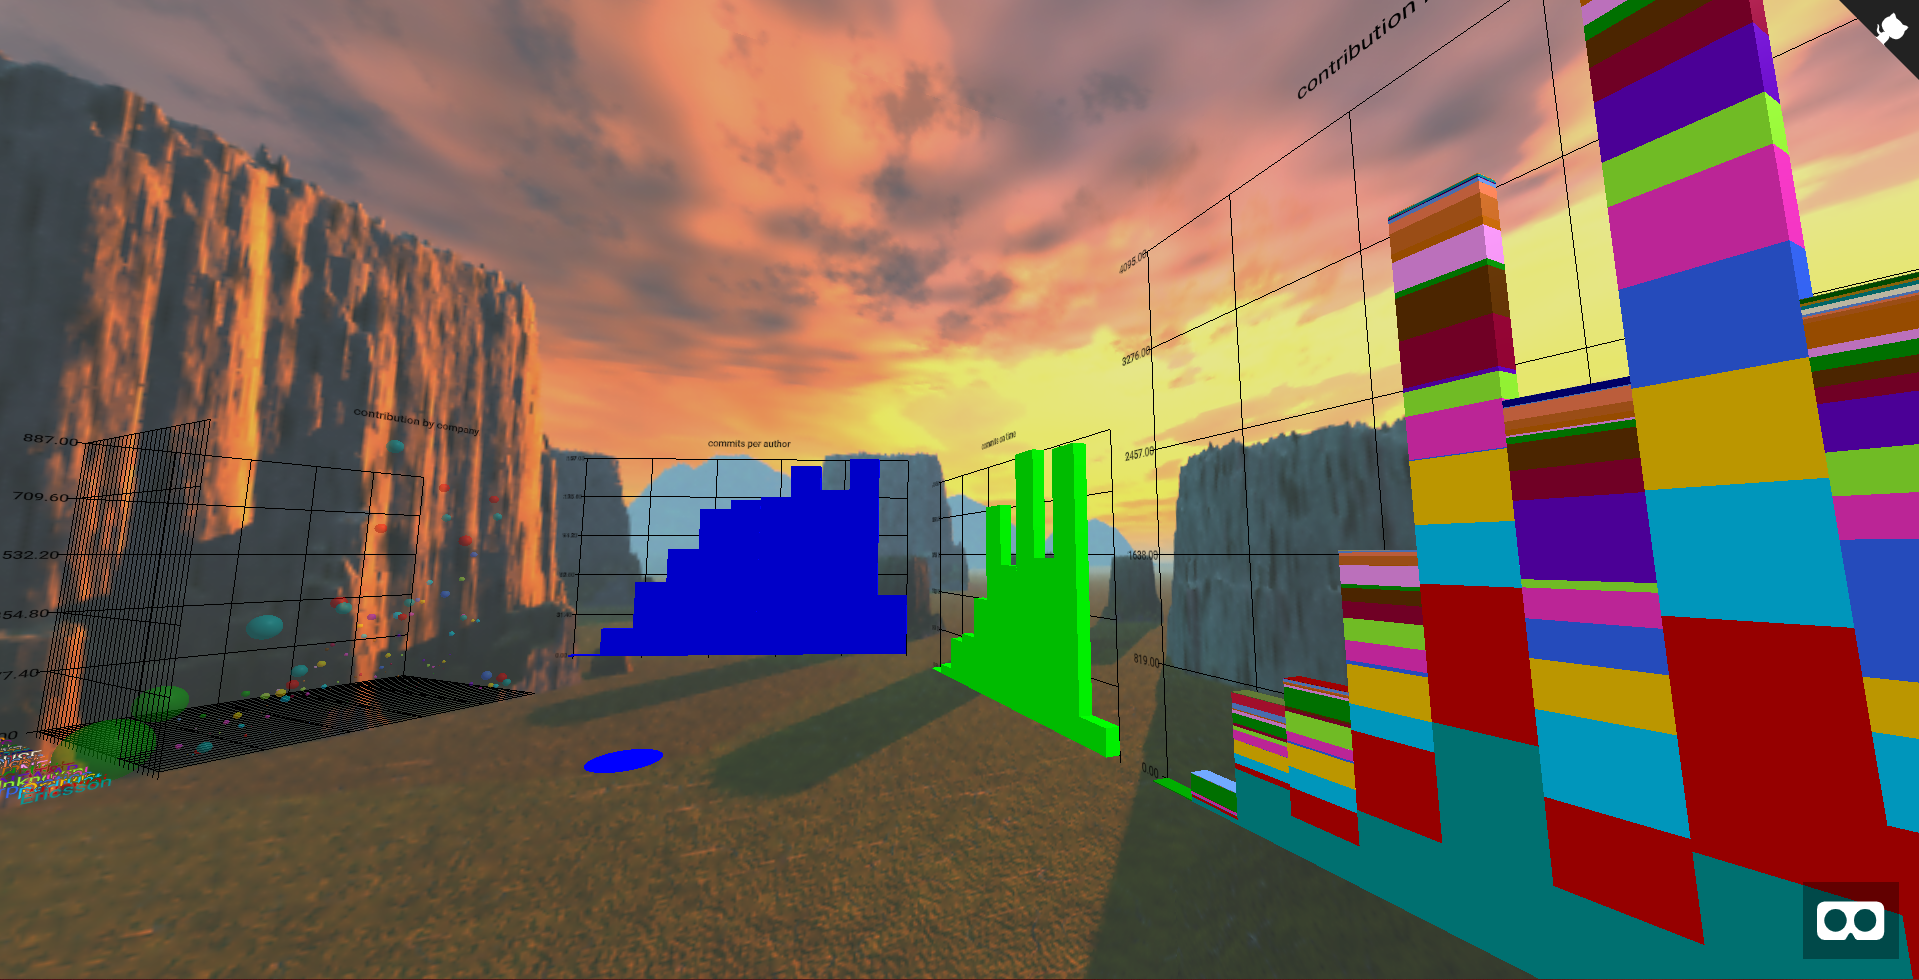
\includegraphics[width=16cm, keepaspectratio]{img/context/aframedc.png}
  \caption{Example of charts with A-FrameDC}
  \label{fig:pluginhtml}
\end{figure}



\section{ThreeDC}
\label{sec:threedc}

ThreeDC\footnote{\url{https://adrianalonsoba.github.io/web-ThreeDC/}} is a library to create different kind of data visualizations based on Three.js\footnote{\url{https://threejs.org/}}. According to the docs that the main developer has, Three.js is a JavaScript library; the aim of the project is to create an easy to use, lightweight, 3D library. The library provides Canvas 2D, SVG, CSS3D and WebGL renderers. It can be defined as "a library to make WebGL easier". 
WebGL is an API. It lets you access a computer's specialised graphics hardware using JavaScript, and render the output to a webpage in a regular old <canvas> element. Before WebGL, access to that specialised hardware was only really doable with desktop software. The browser was stuck in 2D town (excluding third-party plug-ins such as Adobe Flash).
ThreeDC extends by default the API of Three.js encapsulating it in a new API focused on the creation of 3D objects related to data visualization. This way, this type of 3D graphics can be built easily without technical knowledge of Three.js or WebGL. This library allows the creation of graphs of 2D lines with 2 axes, bars in 2D and 3D with 2 or 3 axes (with the probability that they are stacked bars), bubbles with 3 axes and pie charts.

This library has been developed by an ex-student of the URJC being his degree thesis \cite{Threedcmemoria}.

\begin{figure}[H]
  \centering
  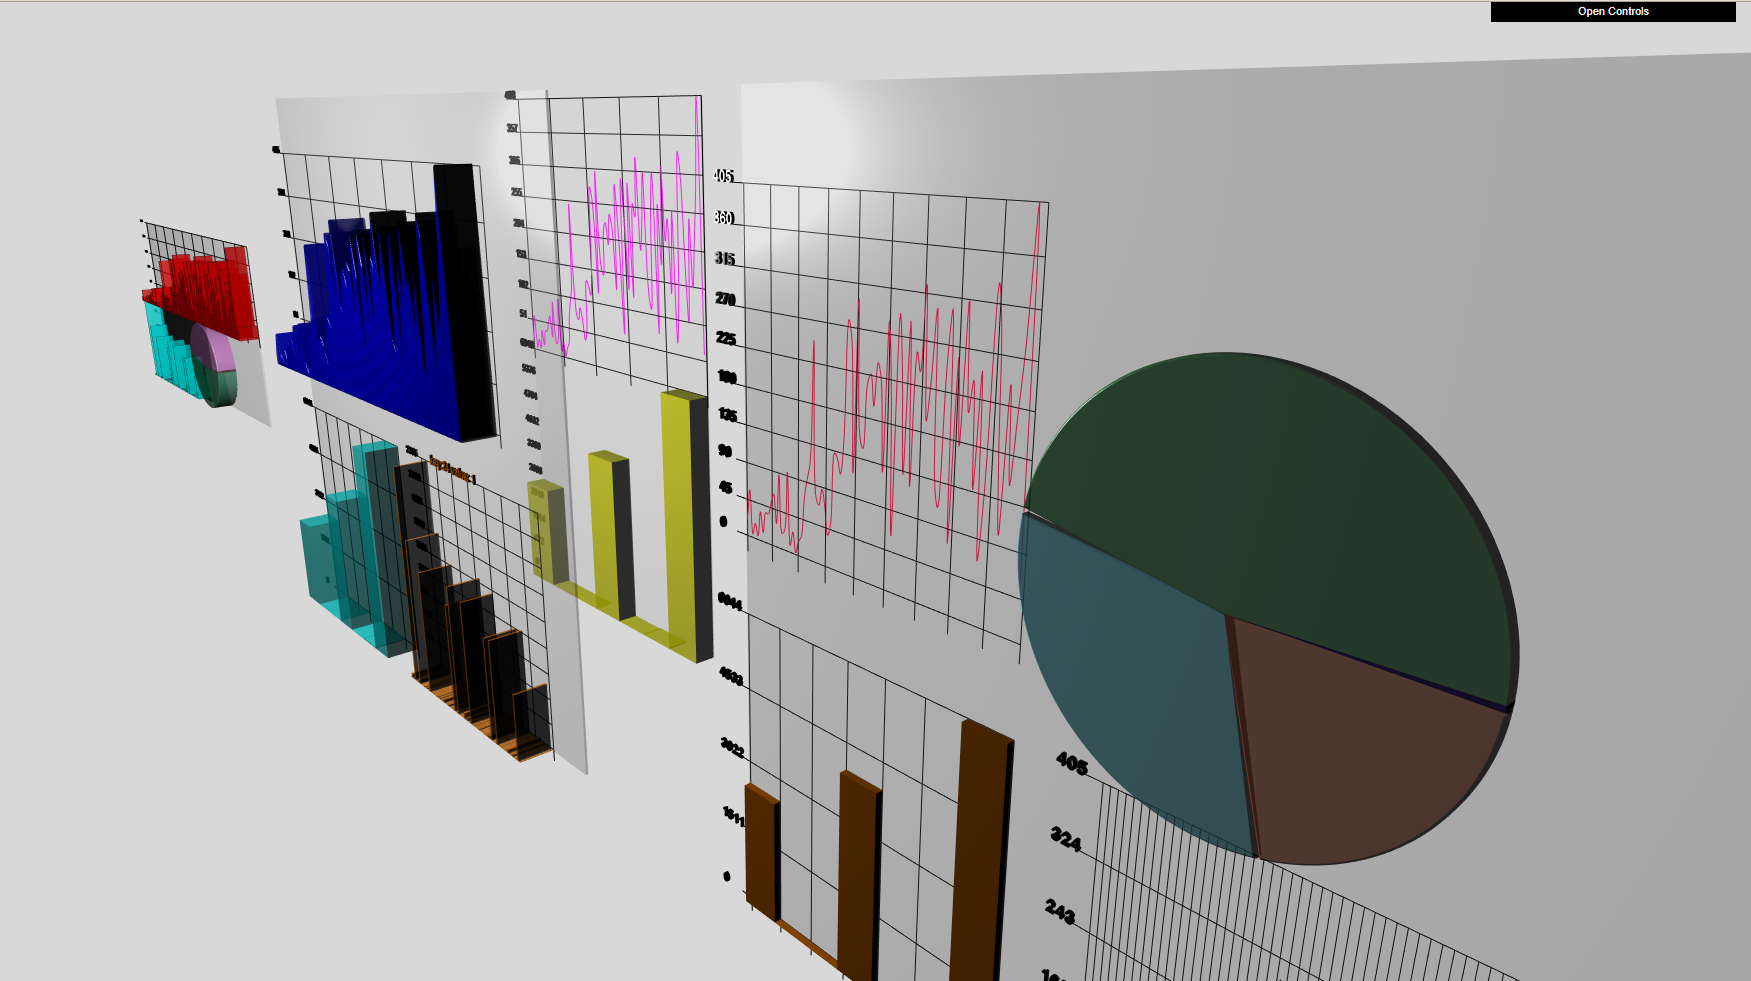
\includegraphics[width=16cm, keepaspectratio]{img/context/threedc.png}
  \caption{Example of charts with ThreeDC}
  \label{fig:pluginhtml}
\end{figure}

\section{AngularJS}
\label{sec:angular}
AngularJS is a structural framework for dynamic web apps. It lets you use HTML as your template language and lets you extend HTML's syntax to express your application's components clearly and succinctly. Angular's data binding and dependency injection eliminate much of the code you would otherwise have to write. And it all happens within the browser, making it an ideal partner with any server technology.

AngularJS teaches the browser new syntax through a construct we call directives. Examples include:

\begin{itemize}
\item Data binding, as in \{\{\}\}.
\item DOM control structures for repeating, showing and hiding DOM fragments.
\item Support for forms and form validation.
\item Attaching new behavior to DOM elements, such as DOM event handling.
\item Grouping of HTML into reusable components.
\end{itemize}

AngularJS is not a single piece in the overall puzzle of building the client-side of a web application. It handles all of the DOM and AJAX glue code you once wrote by hand and puts it in a well-defined structure. This makes AngularJS opinionated about how a CRUD (Create, Read, Update, Delete) application should be built. But while it is opinionated, it also tries to make sure that its opinion is just a starting point you can easily change.

AngularJS simplifies application development by presenting a higher level of abstraction to the developer. Like any abstraction, it comes at a cost of flexibility. In other words, not every app is a good fit for Angular. AngularJS was built with the CRUD application in mind. Luckily CRUD applications represent the majority of web applications. To understand what AngularJS is good at, though, it helps to understand when an app is not a good fit for Angular.

Games and GUI editors are examples of applications with intensive and tricky DOM manipulation. These kinds of apps are different from CRUD apps, and as a result are probably not a good fit for Angular. In these cases it may be better to use a library with a lower level of abstraction, such as jQuery.

VBoard is completely written in AngularJS, so it is used all the syntax and optimum ways of the AngularJS development (directives, scopes, modules, etc.).

\section{NodeJS and Npm}
\label{sec:nodejsnpm}
Node.js is a JavaScript runtime built on Chrome's V8 JavaScript engine. Node.js uses an event-driven, non-blocking I/O model that makes it lightweight and efficient.As an asynchronous event driven JavaScript runtime, Node is designed to build scalable network applications.

Node.js applications are written in JavaScript, and can be run within the Node.js runtime on OS X, Microsoft Windows, and Linux. Node.js also provides a rich library of various JavaScript modules which simplifies the development of web applications using Node.js to a great extent.

\begin{lstlisting}[frame=single]
Node.js = Runtime Environment + JavaScript Library
\end{lstlisting}

Following are the areas where Node.js is proving itself as a perfect technology partner.
\begin{itemize}
\item I/O bound Applications
\item Data Streaming Applications
\item Data Intensive Real-time Applications (DIRT)
\item JSON APIs based Applications
\item Single Page Applications
\end{itemize}


Npm (node package manager) is the package manager for JavaScript. Find, share, and reuse packages of code from hundreds of thousands of developers — and assemble them in powerful new ways. 

The best way to manage locally installed npm packages is to create a package.json file.A package.json file affords you a lot of great things:
\begin{enumerate}
\item It serves as documentation for what packages your project depends on.
\item It allows you to specify the versions of a package that your project can use using semantic versioning rules.
\item Makes your build reproducible which means that its way easier to share with other developers.
\end{enumerate}

As a bare minimum, a package.json must have:
\begin{itemize}
\item "name"
\begin{itemize}
\item all lowercase
\item one word, no spaces
\item dashes and underscores allowed
\end{itemize}
\item "version"
\begin{itemize}
\item in the form of x.x.x
\end{itemize}
\end{itemize}

For example:
\begin{lstlisting}[frame=single]
{
  "name": "my-awesome-package",
  "version": "1.0.0"
}
\end{lstlisting}

The installation of the necessary modules to show the visualization will be done by npm, building its own "package.json" inside the application directory.  Once the file is built indicating the modules to install, they will be downloaded and installed with the statement "npm install" into a "node\_modules" folder for its later use.

\section{Docker}
\label{sec:docker}
The Linux container has become a tool that helps developers and system administrators to test applications or systems in a secure environment equal to the production environment, reducing testing times and adaptations to hardware changes from the test environment to the production. With Docker's technology we can virtualize a Linux with all the applications that we need within our Linux operating system, to "package" it and deploy it in any other Linux by only introducing a couple of commands.

Docker is an open source project with which we can easily create "containers". These Docker containers could be defined as lightweight virtual machines, less demanding with the chips and memories of the equipment where they will be executed.

\subsection{Containers}

They are like a directory, they contain everything necessary for an application to work without accessing a repository external to the container. Each of these is a secure application platform and isolated from the rest that we can find or deploy on the same host machine.


\subsection{Images}

The Docker image could be understood as an OS with installed applications (for example, an OpenSUSE with an office suite). On this basis we can start adding applications that we will need on another computer where we intend to use the image. In addition, Docker offers us a very simple way to update the images we have created, as well as a simple method to create new images. Images are usually defined in "Dockerfile" files with their own syntax.

\subsection{Repositories}

Also known as Docker Registry, they contain images created by users and available to the public. We can find public repositories and totally free or private repositories where we will have to buy the images that we need. These registries allow to develop or to deploy applications in a simple and fast form in base to templates, reducing the time of creation or implementation of applications or systems.



\section{Other Packages Used}
\label{sec:otherspackage}
\subsection{Bodybuilder}
Bodybuilder\footnote{\url{https://bodybuilder.js.org/}} is a small library that makes ElasticSearch queries easier to write, read, and maintain. This library is used in the project for all the queries that are made to ElasticSearch, this way it is not necessary to use an algorithm that builds the JSON of the query. More generic methods of this library are used, building the JSON in a simple and automatic way.


\subsection{Bootstrap}
Bootstrap\footnote{\url{https://getbootstrap.com/}} is an open source toolkit for developing with HTML, CSS, and JS. I used for building entire apps with Sass variables and mixins, responsive grid system, extensive prebuilt components, and powerful plugins built on jQuery. All the distribution of the HTML elements and their matching CSS of VBoard are modulated with Bootstrap.

\subsection{RequireJS}
According to the main page, RequireJS\footnote{\url{https://requirejs.org/}} is a JavaScript file and module loader. It is optimized for in-browser use, but it can be used in other JavaScript environments, like Rhino and Node. Using a modular script loader like RequireJS will improve the speed and quality of your code. The incorporation of APIs, modules and services of the VBoard application is done through the use of RequireJS, thus importing everything necessary.



%%%%%%%%%%%%%%%%%%%%%%%%%%%%%%%%%%%%%%%%%%%%%%%%%%%%%%%%%%%%%%%%%%%%%%%%%%%%%%%%
%%%%%%%%%%%%%%%%%%%%%%%%%%%%%%%%%%%%%%%%%%%%%%%%%%%%%%%%%%%%%%%%%%%%%%%%%%%%%%%%
% DESARROLLO %
%%%%%%%%%%%%%%%%%%%%%%%%%%%%%%%%%%%%%%%%%%%%%%%%%%%%%%%%%%%%%%%%%%%%%%%%%%%%%%%%

\chapter{Development}

In this chapter, we will analyze the use and development of the application from an increasing point of view, guiding the reader through every stage the project has passed, like he/she had developed it him/herself. The development has been carried out increasingly, leading to different kind of prototypes based on the iterations the project has progressed. This format agrees with the methodology SCRUM.

\section{SCRUM methodology}
SCRUM is an iterative and incremental agile software development framework for managing product development. It defines "a flexible, holistic product development strategy where a development team works as a unit to reach a common goal", challenges assumptions of the "traditional, sequential approach" to product development, and enables teams to self-organize by encouraging physical co-location or close online collaboration of all team members, as well as daily face-to-face communication among all team members and disciplines in the project.

A key principle of SCRUM is its recognition that during production processes, the customers can change their minds about what they want and need (often called requirements volatility), and that unpredicted challenges cannot be easily addressed in a traditional predictive or planned manner. As such, SCRUM adopts an empirical approach,accepting that the problem cannot be fully understood or defined, focusing instead on maximizing the team's ability to deliver quickly, to respond to emerging requirements and to adapt to evolving technologies and changes in market conditions.

In SCRUM there are three main roles defined:	

\begin{enumerate}
\item \textbf{Product owner}: The person responsible for maintaining the product backlog by representing the interests of the stakeholders, and ensuring the value of the work the development team does.
\item \textbf{SCRUM master}: The person responsible for the scrum process, making sure it is used correctly and maximizing its benefits.
\item \textbf{Development team}: A cross-functional group of people responsible for delivering potentially shippable increments of product at the end of every sprint.
\end{enumerate}

In our case the product owner and the SCRUM master are represented by the project tutor, so the development team is the project author. Apart from that, we follow the SCRUM methodology faithfully.

A sprint (or iteration) is the basic unit of development in SCRUM. The sprint is a time-boxed effort; that is, it is restricted to a specific duration. The duration is fixed in advance for each sprint and is normally between one week and one month, with two weeks being the most common.

Each sprint starts with a sprint planning event that aims to define a sprint backlog, identify the work for the sprint, and make an estimated commitment for the sprint goal. Each sprint ends with a sprint review and sprint retrospective, that reviews progress to show to stakeholders and identify lessons and improvements for the next sprints.

SCRUM emphasizes working product at the end of the sprint that is really done. In the case of software, this likely includes that the software has been integrated, fully tested and end-user documented.

Sprints or iterations:
\begin{enumerate}
\item \textbf{Iteration 0}: Investigation and preliminary study
\item \textbf{Iteration 1}: Define application structure
\item \textbf{Iteration 2}: First visualizations
\item \textbf{Iteration 3}: Add VBoard state logic into ElasticSearch
\item \textbf{Iteration 4}: Define panels
\item \textbf{Iteration 5}: Dashboards and stand alone mode
\item \textbf{Iteration 6}: Integration with A-FrameDC
\item \textbf{Iteration 7}: Customization and optimization
\item \textbf{Iteration 8}: Dockerize application
\end{enumerate}

%\ref{fig:scrum}
\begin{figure}[!htb]
  \centering
  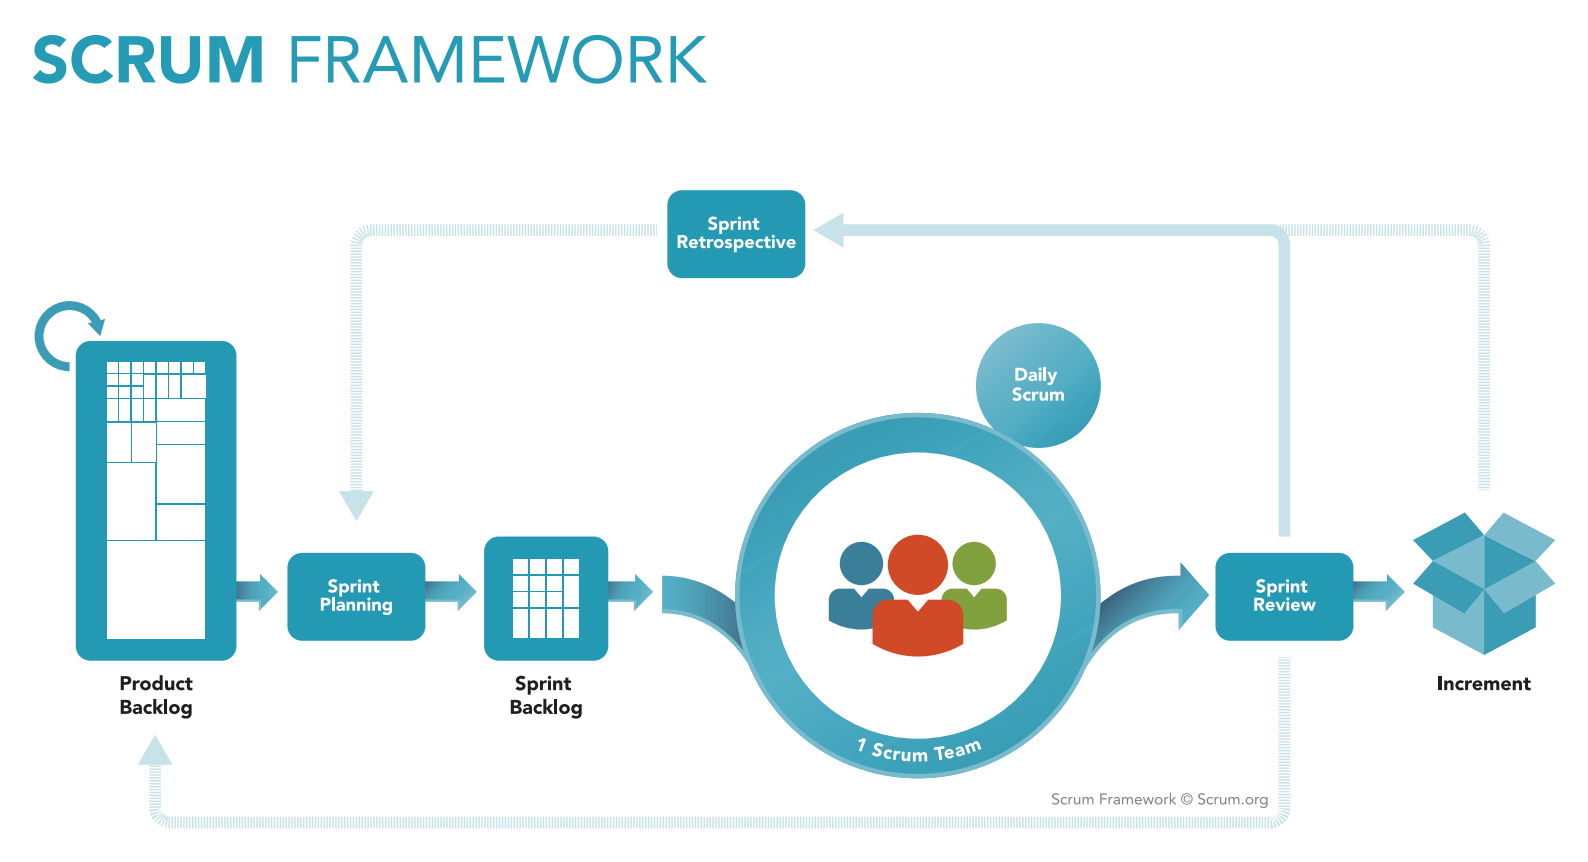
\includegraphics[width=15cm, keepaspectratio]{img/development/SCRUM}
  \caption{The scrum framework}
  \label{fig:scrum}
\end{figure}

\section{Iteration 0: Investigation and preliminary study} 
\label{sec:it0}
This is not an iteration itself, but it is a necessary part of the development, so we decided to include it as 'iteration 0' and here we will get the tools and the study we will need to make our application. 

At the beginning, there were a lot of things to explore. First of all, we have to study, understand and get used to ElasticSearch and a framework in order to develop the application.

During the development of this project, I was working for a company that uses ElasticSearch as a database and search engine, so the study part of ElasticSearch has been easy and it wasn't necessary much time for it. Time has been invested on the study and analysis of ElasticSearch JS API\footnote{\url{https://www.elastic.co/guide/en/elasticsearch/client/javascript-api/current/api-reference-5-6.html}}, a Javascript library to manage the connections and to do all kind of requests to ElasticSearch.

In the choice of the Web development framework, after the experience gained in the development of the degree thesis (Network Plugin)\footnote{\url{https://dlumbrer.github.io/kbn_network/}} it has been decided for the use of AngularJS as a framework, since they have enough knowledge for the full development of the application and therefore the time invested can be allocated to future functionalities of the application.


\section{Iteration 1: Define application structure}
\label{sec:it1}

The aim of this iteration is to define the entire structure, starting with the files structure in order to have isolated each script in a folder that contains scripts with the same type, following the AngularJS standard. Also in this iteration, we are going to define the visual structure, dividing the screen in zones where the items will be, like the menu, the 3D scene, the different pages that it will have, etc.
So we can divide this iteration in this two sub-iterations:

\begin{enumerate}
\item Define the files/scripts structure of the application.
\item Define the visual structure of the application.
\end{enumerate}

\subsection{Files/scripts structure}

To start, the best way to structure an AngularJS application, which as first level scripts, or root, we have a basic \textit{index.html} with very few generic information of the application and a \textit{main.js}, where the Angular application is defined, with the name and path where the code is located.

After, a folder called \textit{app/}, another one \textit{templates/} and another one, \textit{css/}, will be created at the same level, which will contain all the logic developed for the application. Specifically within the \textit{templates/} folder, there will be all the html templates necessary for the application, all the HTML5 code and with names that determine to which zone/section they belong to. Inside the folder \textit{css/} there will be style files to customize and layout the visual aspect of the application. In the \textit{app/} folder there will be all the JavaScript logic developed for the application; in its content it will have a script \textit{app\_module.js} where the AngularJS application is instantiated and its structure is defined, defining the drivers, templates, services and directives you need. In addition, at the same level, there will be three types of folders (if necessary) where the JavaScript scripts corresponding to the directives (folder \textit{directive/}), the JavaScript scripts corresponding to the controllers (folder \textit{controller/}) and the scripts corresponding to the external services of the application (folder \textit{service/}) will be saved.

In addition, there will be a file called \textit{package.json} where the information (metadata) of the project will be defined, as well as the name, author, license, and NPM dependencies needed (libraries), therefore, once the dependencies are installed through "npm install", these will be stored inside the folder \textit{node\_modules/}.

Finally, there will be another folder with the name \textit{js/} where those JavaScript libraries, which are not possible to install using npm (ThreeDC or A-FrameDC, for example) or that have been developed from scratch for this project, will be stored.

With this structure, the development is clean, isolated and easily scalable. The following figure shows the final structure:

\begin{figure}[H]
  \centering
  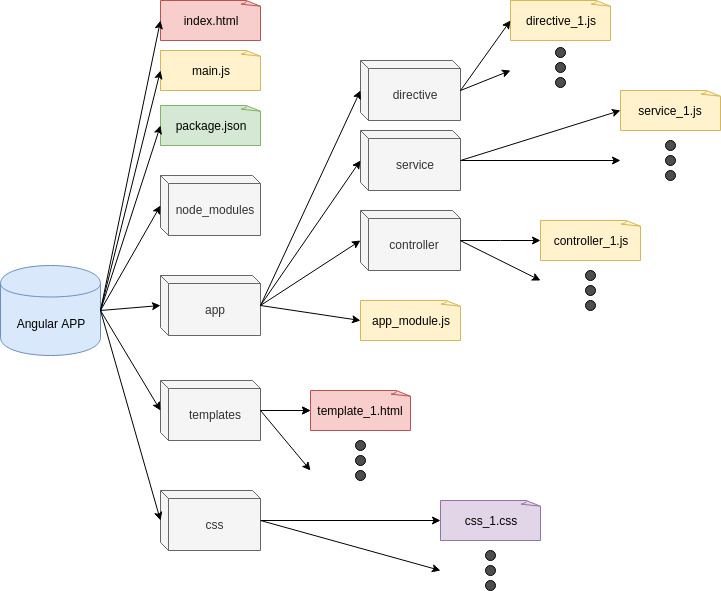
\includegraphics[width=16cm, keepaspectratio]{img/development/Angular_structure}
  \caption{The AngularJS app structure}
  \label{fig:angularjsstructure}
\end{figure}

\subsection{Visual structure}

For the creation of dashboards that visualize data, we have observed applications such as Kibana, Grafana, Freeboard, etc. to follow a similar creation process: easy and understandable for any user. To do this, the creation flow of a dashboard will be create one or more visualizations, optionally create panels containing one or more visualizations and then add these visualizations to a dashboard, so that finally the dashboard contains all the information that wants to be visualized in a 3D and VR environment.

\begin{figure}[H]
  \centering
  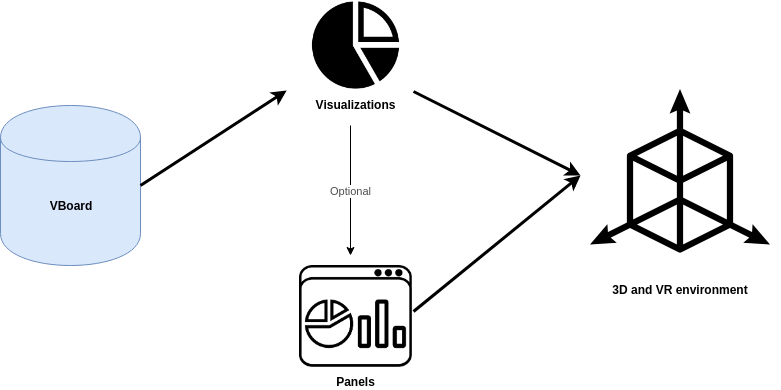
\includegraphics[width=16cm, keepaspectratio]{img/development/Workflow}
  \caption{Create a Dashboard workflow}
  \label{fig:dashboardworkflow}
\end{figure}

Therefore, to follow this workflow, 3 "tabs" or "areas" have been defined in the application: Visualize, Panels, Dashboard and Show:
\begin{enumerate}
    \item \textbf{Visualize}: Section where the visualizations will be created, it will be possible to choose between different types of 3D visualization and in this part it will be chosen which types of data the visualization will show. The visualizations can be saved in order to load/modify them.
    \item \textbf{Panels}: Section where panels will be created, external flat walls that contain visualizations, in this section it can be defined the size of the panel and the number of visualizations that it will contain (by rows and columns); also, the available visualizations should appear to be able to add them to the panel. The panels can be stored in order to load/modify them.
    \item \textbf{Dashboard}: Section where the final "product" will be created, a dashboard that will be a 3D scene where previously saved visualizations and/or panels can be included, so a list of the available visualizations/panels must appear to place them anywhere in the scene, so the user should choose at what point of the scene he/she wants to place the visualization/panel and what rotation it will have. These dashboards must be able to be saved in such a way that they can be loaded in another section in order to visualize them, navigate among them and modify them.
    \item \textbf{Show}: This section will show a list of available dashboards, each with a link to a new resource in which only the 3D scene will appear with a possible VR button to visualize the dashboard in "stand alone" mode without any control in the screen, just to observe data and/or navigate through them with VR.
\end{enumerate}

The navigation amongst these three areas will be through a global navigation bar located at the top of the application. This navigation bar will be shown in each and every one of the sections except for Show since, as it was previously explained, it is only to visualize the dashboard without any control around. Besides, this navigation bar will remain with a "hold" in the section that is in that moment.

\begin{figure}[H]
  \centering
  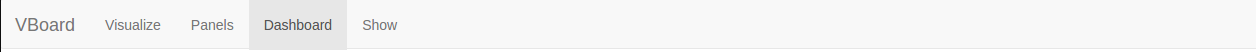
\includegraphics[width=16cm, keepaspectratio]{img/development/navbar}
  \caption{Navbar of VBoard}
  \label{fig:pluginhtml}
\end{figure}

For the modeling of the visual structure, the bootstrap library has been used so that the content can be easily divided into rows and columns of a certain width, this way the content of the Visualize, Panels and Dashboard sections has been structured as a content of two columns, as seen in the following image:

\begin{figure}[H]
  \centering
  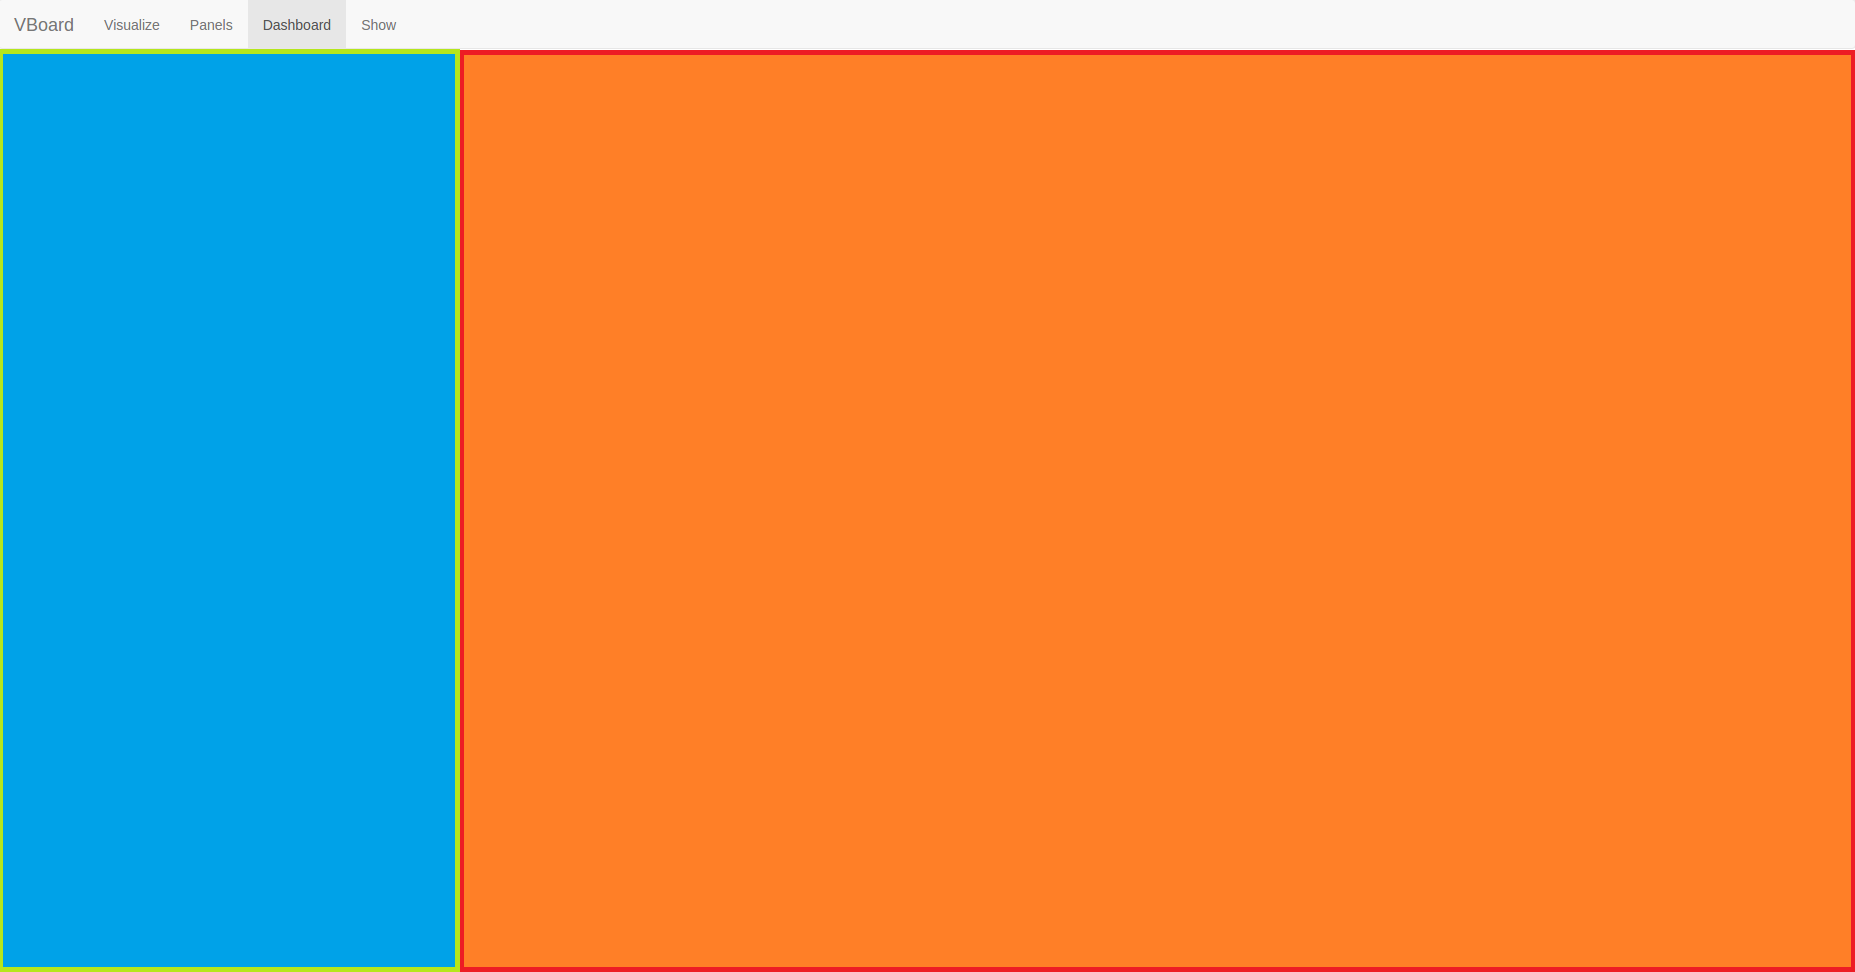
\includegraphics[width=16cm, keepaspectratio]{img/development/visualstructure}
  \caption{Visual Structure of Visualize, Panels and Dashboards}
  \label{fig:pluginhtml}
\end{figure}

The column on the left, green and blue of smaller size corresponds to the control area of the section, that is, where the controls to create, provide data and modify the display/panel/dashboard will be. The orange one will correspond to the 3D scene where the visualizations/panels/dashboards will be visualized. Optionally, a button that changes to VR mode can be added.

In contrast, the Show section will only have a content in which there will be a list with the available dashboards; once an item in the list is clicked, a scene will appear in the whole screen, without the navigation bar or control area:

\begin{figure}[H]
  \centering
  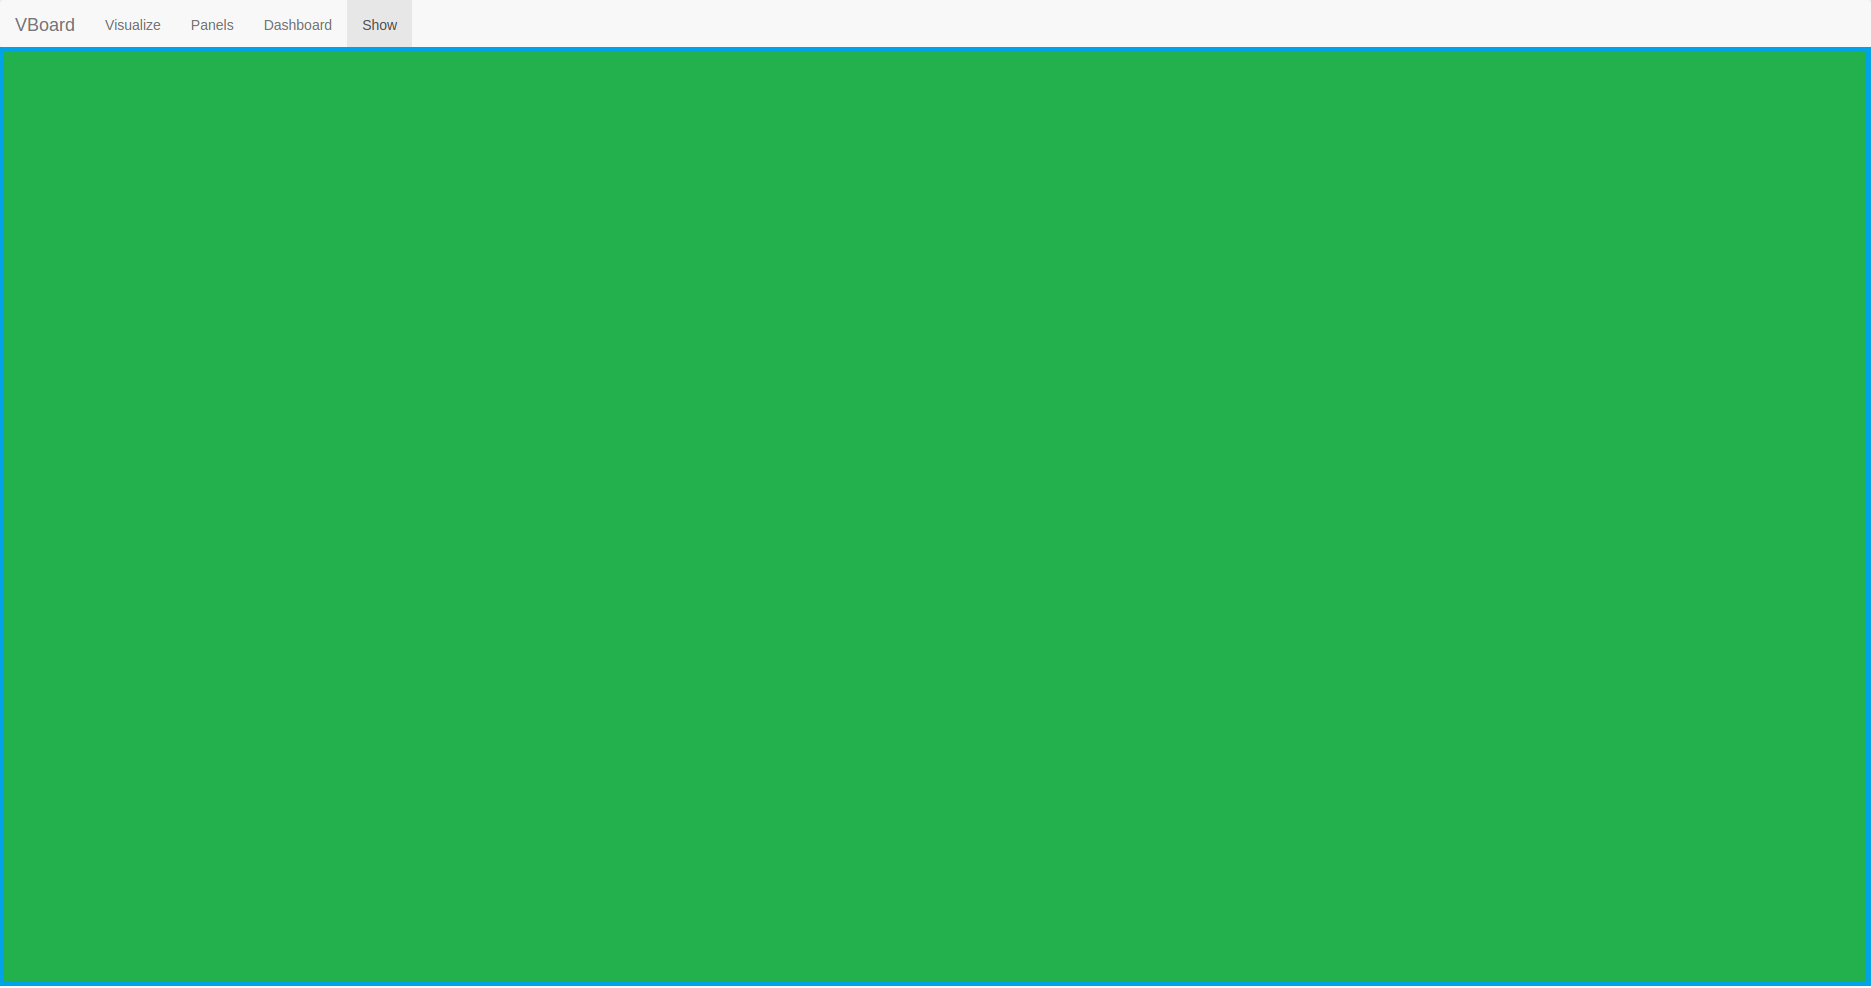
\includegraphics[width=16cm, keepaspectratio]{img/development/showstructure}
  \caption{Visual Structure of Show}
  \label{fig:pluginhtml}
\end{figure}

\section{Iteration 2: First visualizations}

Once we have defined the files structure and developed the visual structure, the next step is to start creating visualizations in the "Visualize" tab for its later integration in a dashboard. Therefore, the aims of this iteration are:

\begin{enumerate}
\item First visualizations without data
\item Integration with ElasticSearch
\item Development of the control menu
\item APIs in order to query easy ElasticSearch
\end{enumerate}

\subsection{Visualizations without data}

To begin with, with the aim of get used to and know how to use the ThreeDC library, some simple visualizations in the visualization part were created, without any data from ElasticSearch; some test data in the code were used. Luckily, the author of the library has several examples on his web\footnote{https://adrianalonsoba.github.io/web-ThreeDC/}, therefore, it only has be adapted these examples to VBoard. The following screenshots show some of the visualizations that have been tested within VBoard:



\begin{figure}[H]
 \centering
  \subfloat[Example of visualizations]{
    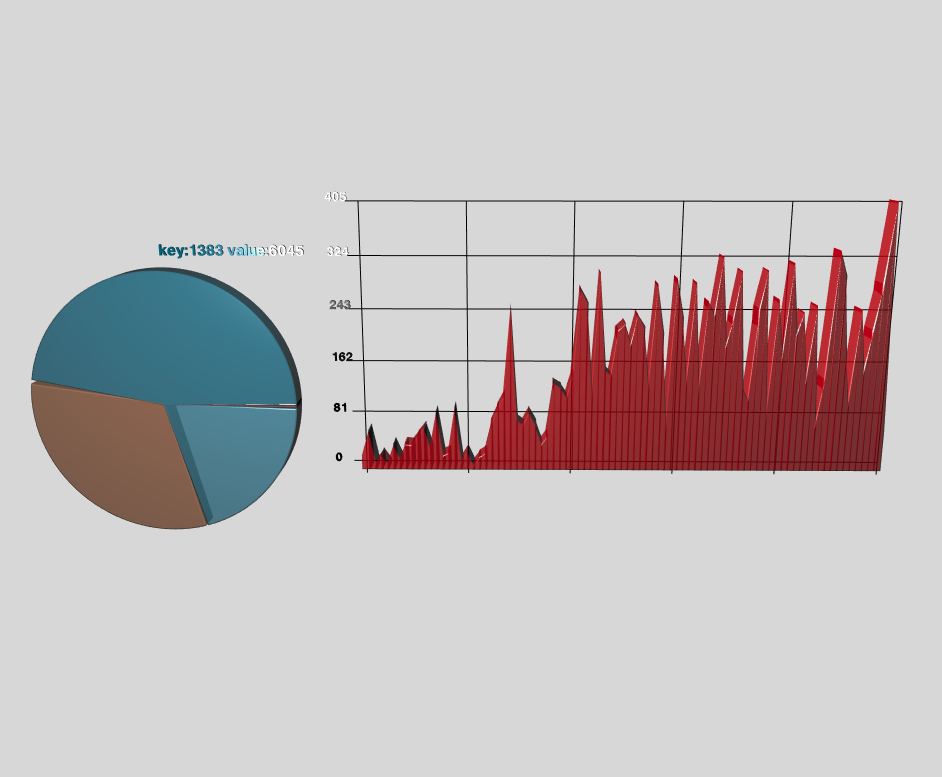
\includegraphics[width=0.5\textwidth]{img/development/example1}}
  \subfloat[Example of panel]{
    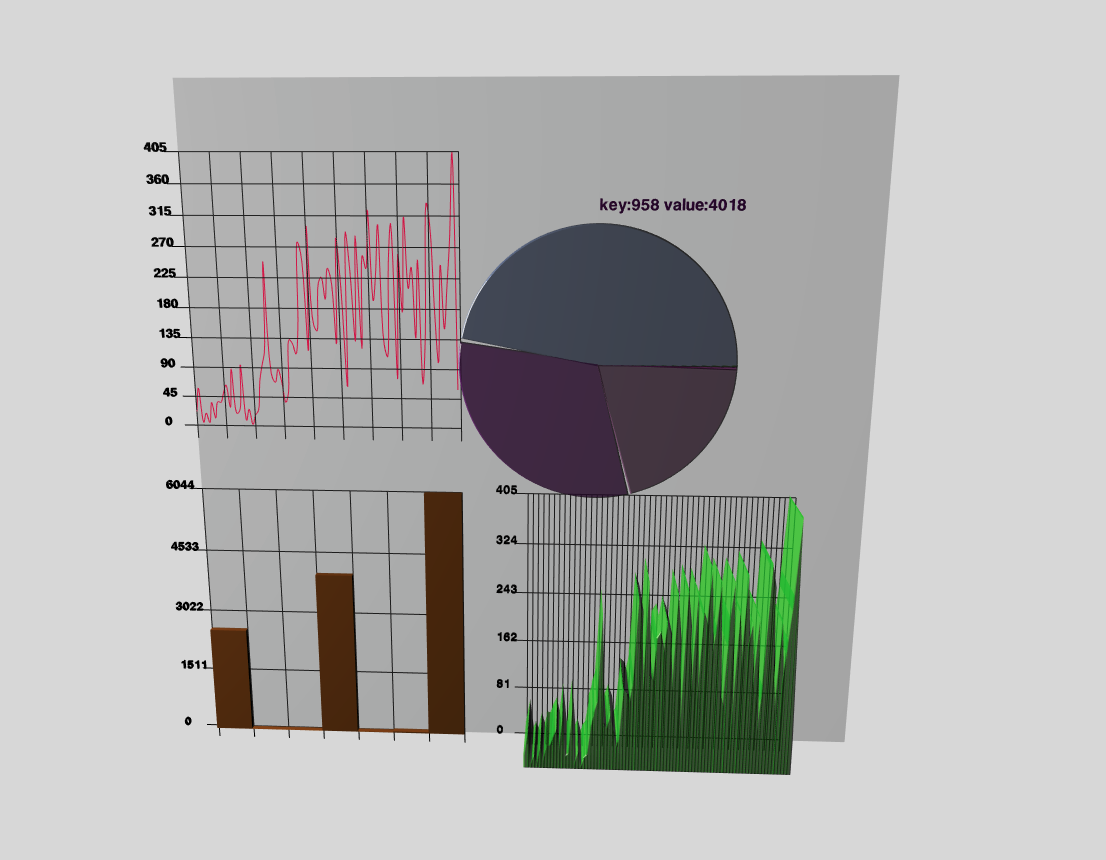
\includegraphics[width=0.5\textwidth]{img/development/example2}}
 \caption{Example of ThreeDC visualizations}
 \label{f:threedcexamples}
\end{figure}

It's necessary to keep in mind that these examples are a creation of a scene by adding simple elements that can be created with ThreeDC. In none of the cases the data come from a data source, this will be the next objective.

\subsection{Integration with ElasticSearch}

For the integration of ElasticSearch, as it was told in the section \ref{sec:elasticsearch}, ElasticSearch will be used as a database to create visualizations, so in this application it will be integrated as a service, creating its file \textit{ESService.js} in the corresponding folder \textit{app/service/} of VBoard; inside this file, the ElasticSearch service is instantiated, defining a client by this address, by default localhost:9200:

\begin{lstlisting}[frame=single]
define([], function () {
  function ESService(esFactory) {
    this.client = esFactory({
      host: 'http://localhost:9200',
    });
  }
  return ESService;
});
\end{lstlisting}

With this instantiated service, we can include the client to ElasticSearch in any controller that we use in the application, therefore, in the controller of the "Visualize" tab it will be included, in such a way that we can create visualizations with ElasticSearch data in real time..

We can only make queries to ElasticSearch using this service and the JavaScript API that they have published \footnote{\url{https://www.elastic.co/guide/en/elasticsearch/client/javascript-api/current/api-reference-5-6.html}}. The next problem was the construction of this query, the part inside the body, where the aggregations that are going to be searched in ElasticSearch are defined.

To solve this problem the bodybuilder\footnote{\url{https://bodybuilder.js.org/}} library has been used to make these aggregations and build the object that goes into the query in a simple way. Anyway, we discovered that the code is hard and complex to use the library directly, so we decided to create from scratch two internal APIs, genES and buildESDS, to make the calls to ElasticSearch and to create the object that goes inside the query using bodybuilder.

\subsubsection{buildESDS}
This API is located in the \textit{js/} folder and it is basically responsible for saving the selected aggregations, it consists of a few methods, to add metrics and buckets, to build that object (data structure) and to return it.

\subsubsection{genES}
This API is in the \textit{js/} folder and this API is responsible for creating the object that goes inside the body of the query to ElasticSearch using the bodybuilder library and the object of the previous API (buildESDS) until making all the requests to ElasticSearch, returning promises to then work with the returned data. It is the core of everything related to queries to ElasticSearch. It consists of several methods, from building the bodybuilder object to all the necessary requests.


\subsection{Development of the control menu}

Once the APIs and everything necessary to make requests to ElasticSearch have been created, the next step is to create a menu in the control area in order to configure the data that we want to visualize as well as what kind of visualization we want. The menu has been developed using bootstrap elements to be useful and to have a simple interface and that anyone can understand. Therefore, steps similar to those of the Kibana application have been defined to build a visualization:

\begin{enumerate}
    \item Index and type selection: the first thing is to choose on what index and type of our ElasticSearch we will want to show the data, there will be two dropdowns and we will have to choose first the index to be able to visualize something in de type. To continue, there is also a button called "Show Mapping" to optionally see the mapping that the chosen index has:
        \begin{figure}[H]
          \centering
          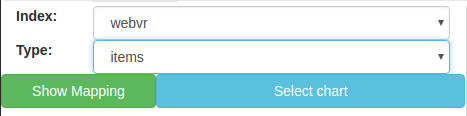
\includegraphics[width=10cm, keepaspectratio]{img/development/indextype}
          \caption{Index/type selection}
          \label{fig:index-type}
        \end{figure}
    \item Visualization type: A dropdown in order to select the different kinds of visualization that will be in VBoard, to continue we have to click on Select Data (or cancel if we want to go back):
        \begin{figure}[H]
          \centering
          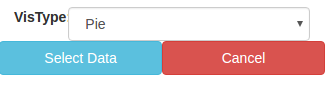
\includegraphics[width=8cm, keepaspectratio]{img/development/vistype}
          \caption{Index/type selection}
          \label{fig:vistype}
        \end{figure}
    \item Select data: Like the Kibana application, this is where the metrics and buckets that will add the data to be displayed are chosen, the amount of metrics and buckets needed to display the visualization will vary depending on the type of visualization, there will be several dropdowns to choose the type of metric/bucket and the field to which it will add:
    \begin{figure}[H]
      \centering
      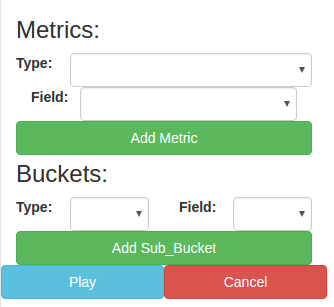
\includegraphics[width=8cm, keepaspectratio]{img/development/aggregationstype}
      \caption{Data selection}
      \label{fig:aggregationstype}
    \end{figure}
\end{enumerate}

Once all the above has been selected, play will be pressed and internally, VBoard will generate all the queries and it will show, as a result, the visualization, for example:

\begin{figure}[H]
  \centering
  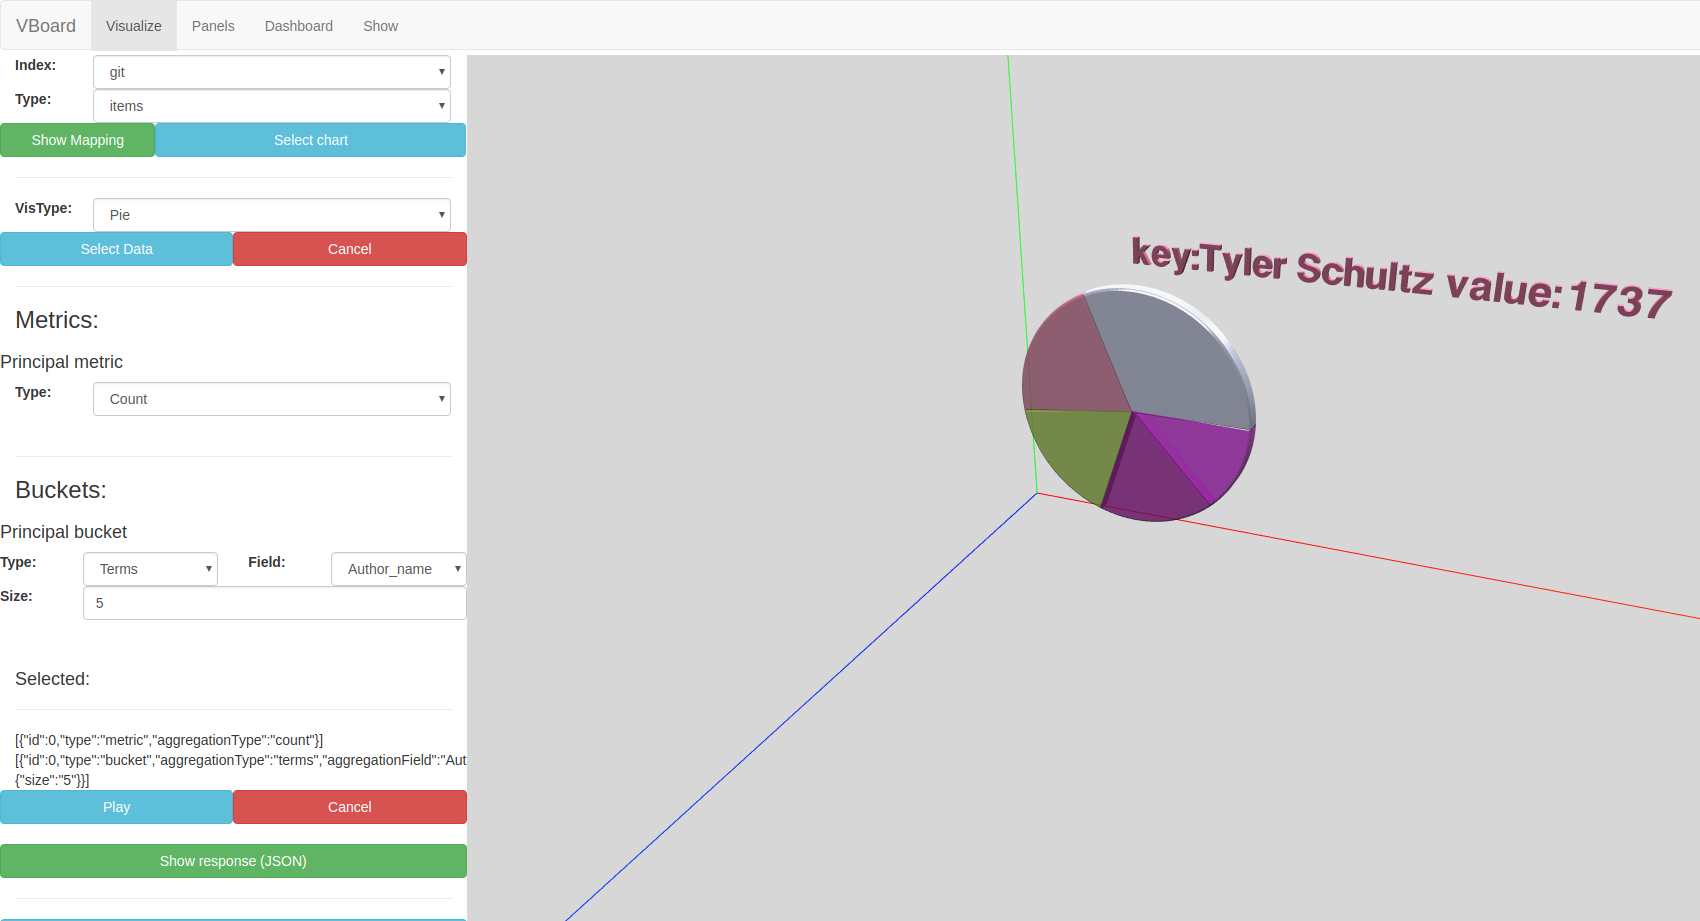
\includegraphics[width=16cm, keepaspectratio]{img/development/firstdatavisualization}
  \caption{First data visualization}
  \label{fig:firsdatavisualization}
\end{figure}

Optionally there will be a button called "Show response (JSON)" so that the result of the data that has been requested to ElasticSearch (both aggregated and in raw) to show the visualization, can be seen.


\section{Iteration 3: Add VBoard state logic into ElasticSearch}

The next step to build panels and dashboards, is to have a logic and a storage system in ElasticSearch to be able to save our visualizations. To do this, in this iteration we have defined a new index called ".vboard" where everything related to VBoard will be saved. Specifically in this index the visualizations, panels and dashboards that have been created, will be saved.

To define an index in ElasticSearch, the first thing to do is define the mapping of types and fields that it will have, in this case we have defined 3 different types within the new index ".vboard" in order to have visualizations, panels and dashboards stored in a different type. Each document saved in each of these types has different fields since it is necessary to distinguish that each VBoard object is different.

Once the properties that wants to be stored are defined, the ".vboard" index is the following:

\begin{lstlisting}[frame=single]
PUT .vboard
{
    "settings" : {
        "number_of_shards" : 1
    },
    "mappings" : {
        "visthreed" : {
            "properties" : {
                "chartType" : { "type" : "text" },
                "name" : { "type" : "text" },
                "description" : { "type" : "text" },
                "indexOfES" : {"type" : "text"},
                "typeOfES" : {"type": "text"},
                "metricsSelected" : { "type": "object" },
                "bucketsSelected" : { "type": "object" },
                "data" : { "type": "object" }
            }
        },
        "panelthreed" :  {
          "properties": {
                "position" : { "type" : "text" },
                "rows" : { "type" : "text" },
                "columns" : { "type" : "text" },
                "dimension" : { "type" : "text" },
                "opacity" : { "type" : "text" },
                "charts" : { "type" : "object" },
                "name" : { "type" : "text" },
                "description" : { "type" : "text" }
          }
        },
        "dashthreed" : {
            "properties" : {
                "background": { "type": "text"},
                "panels" : { "type" : "object" },
                "charts" : { "type" : "object" },
                "name" : { "type" : "text" },
                "description" : { "type" : "text" }
            }
        }
    }
}
\end{lstlisting}

All the save and edited logic of the VBoard elements has been added to the genES API.

In the graphical part, a logic has been developed to save the visualizations, adding a save button that opens a "modal" in bootstrap with a form to add title and description to the visualization to save:

\begin{figure}[H]
  \centering
  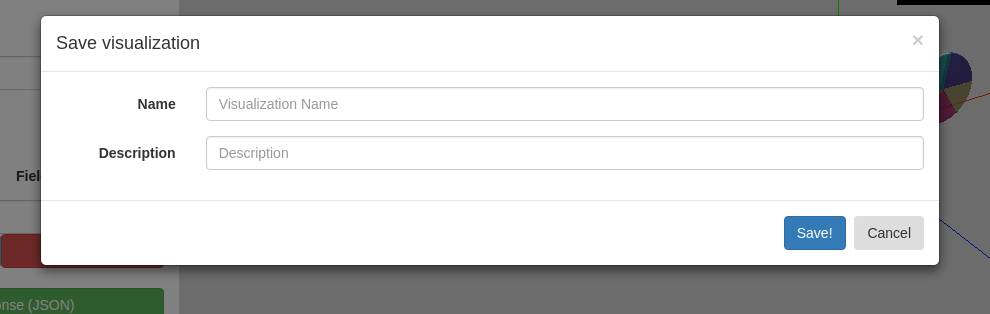
\includegraphics[width=16cm, keepaspectratio]{img/development/examplesave}
  \caption{Form save visualization}
  \label{fig:examplesave}
\end{figure}

This way, the visualization will be saved with a name and description. In the case that there is a visualization with the same name and type, a form will appear asking if we really want to overwrite the visualization.

To edit a saved visualization, we have also developed a loading button that shows a list of the visualizations to load:

\begin{figure}[H]
  \centering
  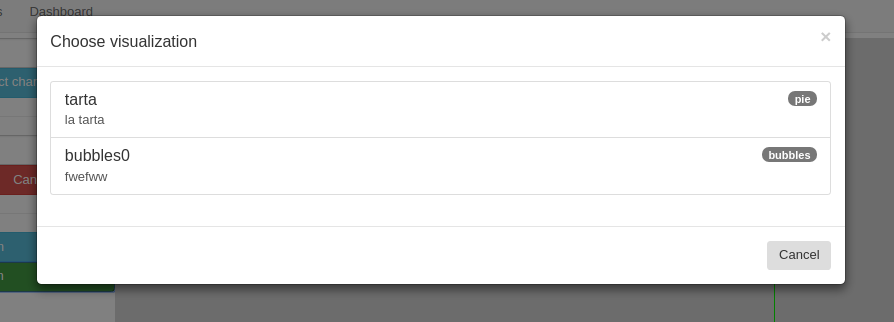
\includegraphics[width=16cm, keepaspectratio]{img/development/exampleload}
  \caption{Form load visualization}
  \label{fig:exampleload}
\end{figure}

Once clicked, the visualization with the selected data will be shown in order to edit it or save it as a new one.

\section{Iteration 4: Define panels}

The next step is to define the panels, their construction and later save/edit logic. The panels are a bit ambiguous concept, in the 3D environment we could call it a "wall" in which "visualizations" are placed. We have put this implementation because the creator of the ThreeDC library has it included in its API.

A panel is defined by width, height, opacity and by the size of visualizations that can be placed on it. By default, an empty panel with a defined opacity and size will appear, but a button called "New Panel" will be find to build it from scratch.

Therefore, in the control menu there is a list with the available visualizations to add to the panel, showing the type of visualization that it is and its title and description. Once an item is clicked, a simple form appears to define where in the panel you want to place the visualization, since it is divided by cells, so you have to select a row and column where you want to place the visualization:

\begin{figure}[H]
 \centering
  \subfloat[Example of visualizations available]{
    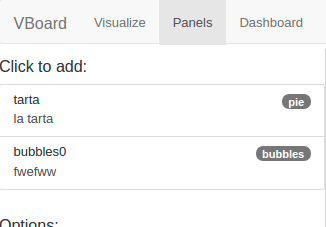
\includegraphics[width=0.3\textwidth]{img/development/panelvislist}}
  \subfloat[Example of add vis to panel form]{
    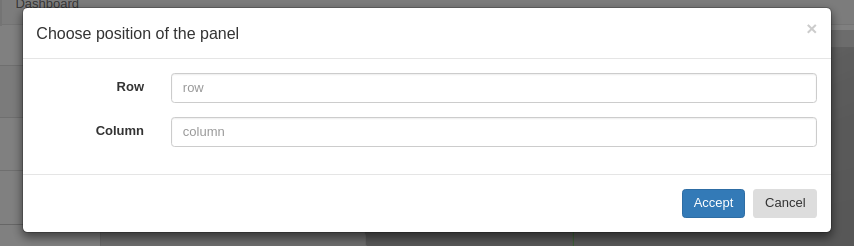
\includegraphics[width=0.7\textwidth]{img/development/exampleaddvistopanel}}
 \caption{Add visualization to a panel}
 \label{f:threedcexamples}
\end{figure}

Below this list of available visualizations, there will be the "New Panel", "Load Panel" and "Save Panel" buttons:

\begin{figure}[H]
  \centering
  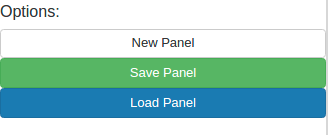
\includegraphics[width=6cm, keepaspectratio]{img/development/panelsbuttons}
  \caption{Options buttons of Panels}
  \label{fig:panelsbuttons}
\end{figure}

As it was explained, clicking on "New Panel" will open a new form to reset the current panel and start a new one. This is the form to start a panel with its characteristics:

\begin{figure}[H]
  \centering
  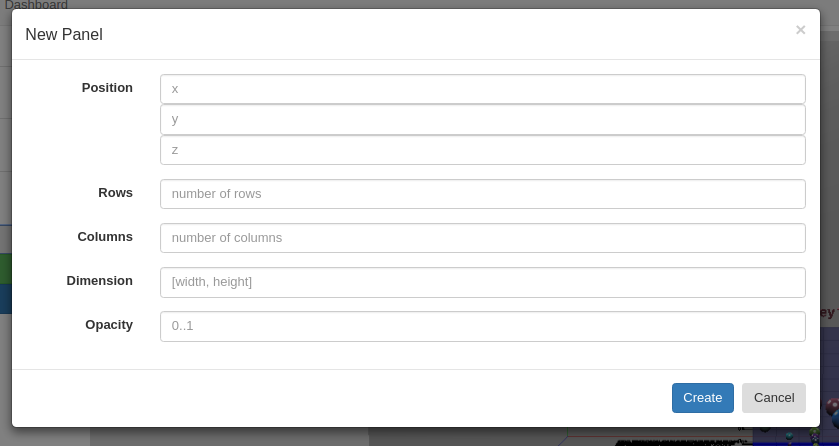
\includegraphics[width=16cm, keepaspectratio]{img/development/newpanelmodal}
  \caption{New Panel Modal}
  \label{fig:newpanelmodal}
\end{figure}

In the case of clicking on "Save Panel", as in Visualize, a modal will open with a form to add title and description to the panel, later it will be saved in ElasticSearch:

\begin{figure}[H]
  \centering
  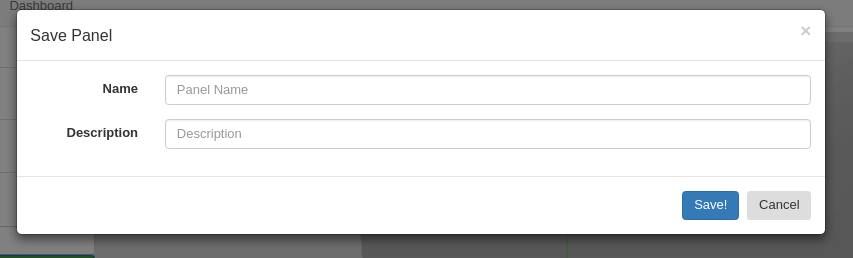
\includegraphics[width=16cm, keepaspectratio]{img/development/savepanelmodal}
  \caption{Save Panel Modal}
  \label{fig:savepanelmodal}
\end{figure}

And finally, the "Load Panel" button will show another modal with the list of available panels, showing the title/description and number of the charts it contains, in order to load and edit them, once it is clicked, it will load itself and all its content for later editing or saving as a new one:

\begin{figure}[H]
  \centering
  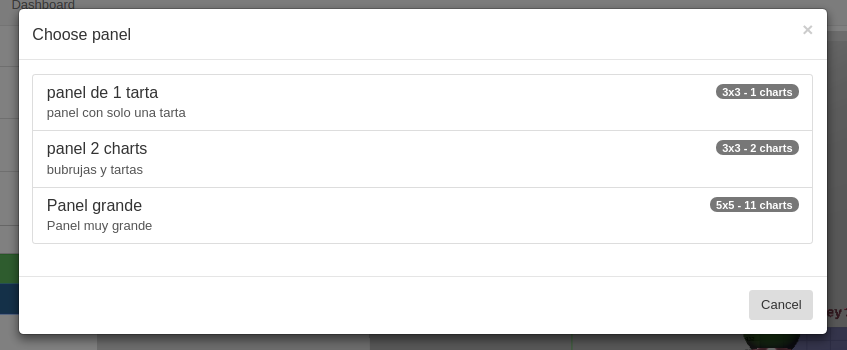
\includegraphics[width=16cm, keepaspectratio]{img/development/loadpanelmodal}
  \caption{Load Panel Modal}
  \label{fig:loadpanelmodal}
\end{figure}

With all this implemented, with its corresponding functions for saving and loading in genES, we will develop the Dashboard tab.

\begin{figure}[H]
  \centering
  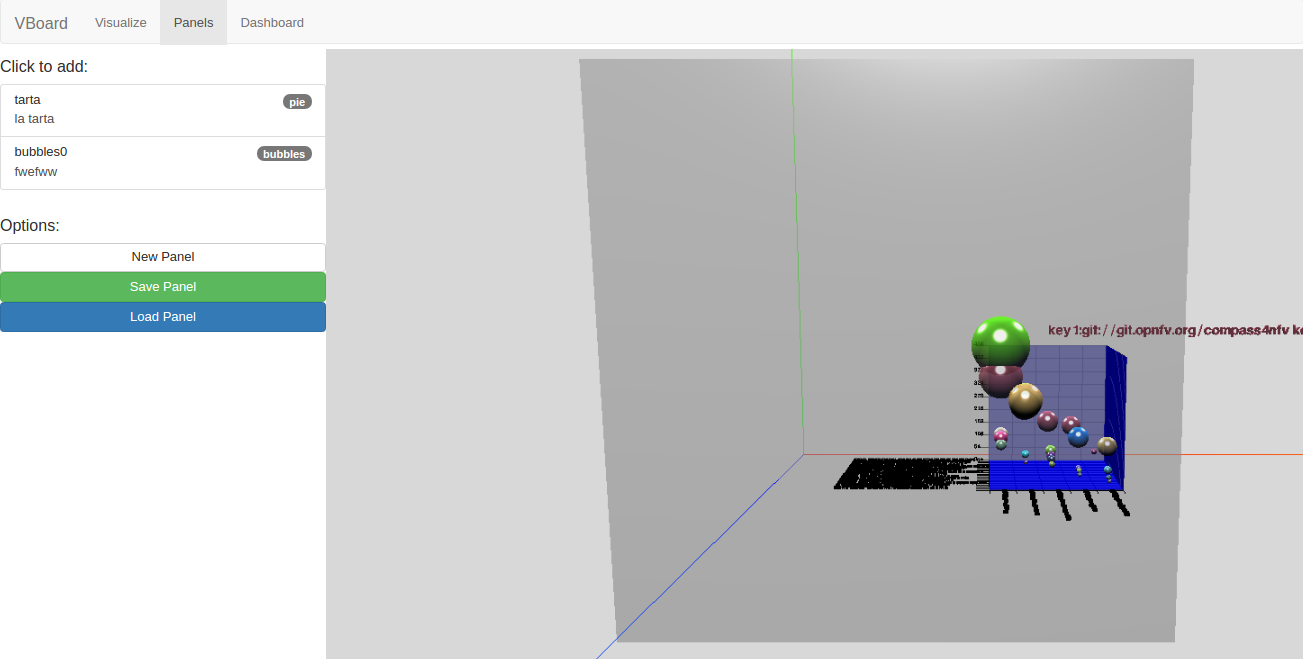
\includegraphics[width=16cm, keepaspectratio]{img/development/examplepanelbubbles}
  \caption{Example of panel with one visualization inside}
  \label{fig:examplepanelbubbles}
\end{figure}

\section{Iteration 5: Dashboard and stand alone mode}

This iteration is divided into 2 subiterations:

\begin{enumerate}
    \item Define dashboards
    \item Show dashboard in stand alone version
\end{enumerate}

\subsection{Define dashboards}

The process of creating a dashboard is the same as the panel; there must be a list of elements that can be added, which in this case are panels and visualizations and there must be able to be added in any position of the 3D scene. By default an empty scene will appear without visualizations.


Therefore, in the control menu there is a list with the visualizations and panels available to add to the panel, showing the type of visualization that it is and its title and description. Once an item is clicked, a simple form appears to define where in the scene you want to place the item, since it has both "x", "y" and "z" axis, so you have to select three positions:

\begin{figure}[H]
 \centering
  \subfloat[List of available items]{
    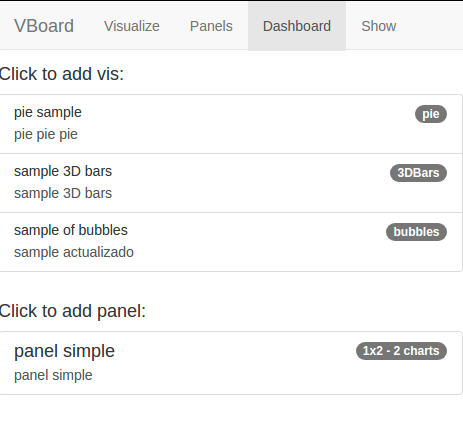
\includegraphics[width=0.3\textwidth]{img/development/addvispaneldashboard}}
  \subfloat[Example of add vis/panel to dashboard form]{
    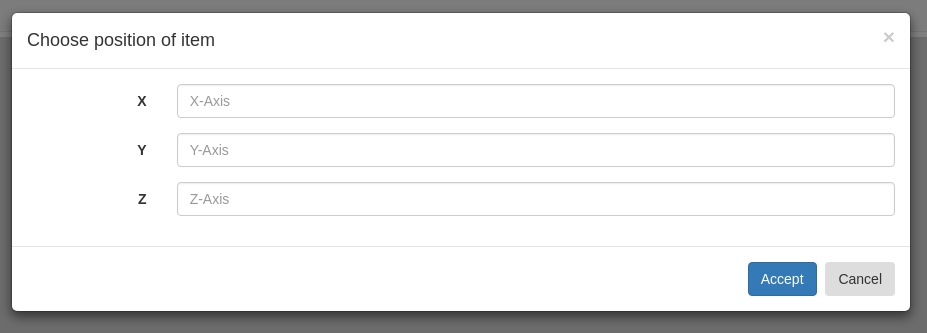
\includegraphics[width=0.7\textwidth]{img/development/exampleaddvistodash}}
 \caption{Add visualization or panel to a dashboard}
 \label{f:threedcexamples}
\end{figure}

Below this list of available visualizations and panels, the "Save Dashboard" and "Load Dashboard" buttons will be found:

\begin{figure}[H]
  \centering
  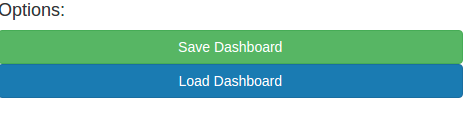
\includegraphics[width=6cm, keepaspectratio]{img/development/dashbuttons}
  \caption{Options buttons of Dashboard}
  \label{fig:dashbuttons}
\end{figure}

In the case of clicking on "Save Dashboard", just like in Visualize, a modal will be opened with a form to add title and description to the dashboard, later it will be saved in ElasticSearch:

\begin{figure}[H]
  \centering
  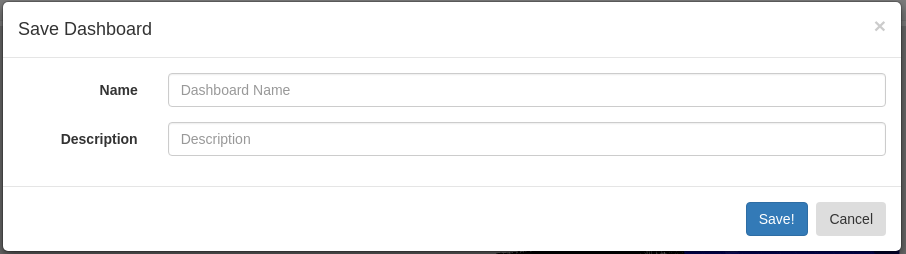
\includegraphics[width=16cm, keepaspectratio]{img/development/examplesavedash}
  \caption{Save Dashboard Modal}
  \label{fig:examplesavedash}
\end{figure}

And finally, the button "Load Dashboard", will show another modal with the list of saved dashboards, showing the title/description and number of charts and panels it contains, to be able to load and edit them, once it is clicked, it will be loaded and all its content for later editing or saving as a new one:

\begin{figure}[H]
  \centering
  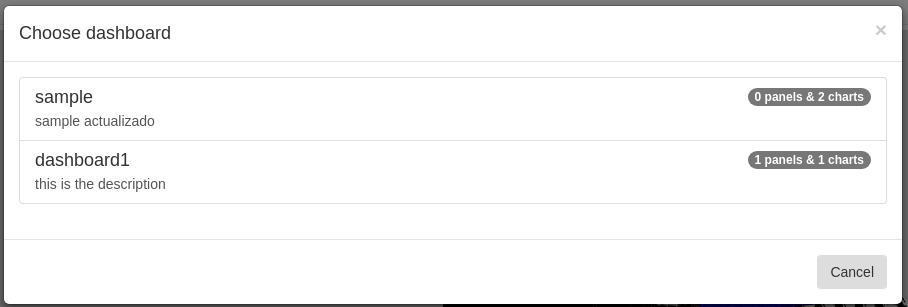
\includegraphics[width=16cm, keepaspectratio]{img/development/exampleloaddash}
  \caption{Load Dashboard Modal}
  \label{fig:exampleloaddash}
\end{figure}

With all this implemented, with its corresponding functions for saving and loading in genES, we will develop the Show tab

\begin{figure}[H]
  \centering
  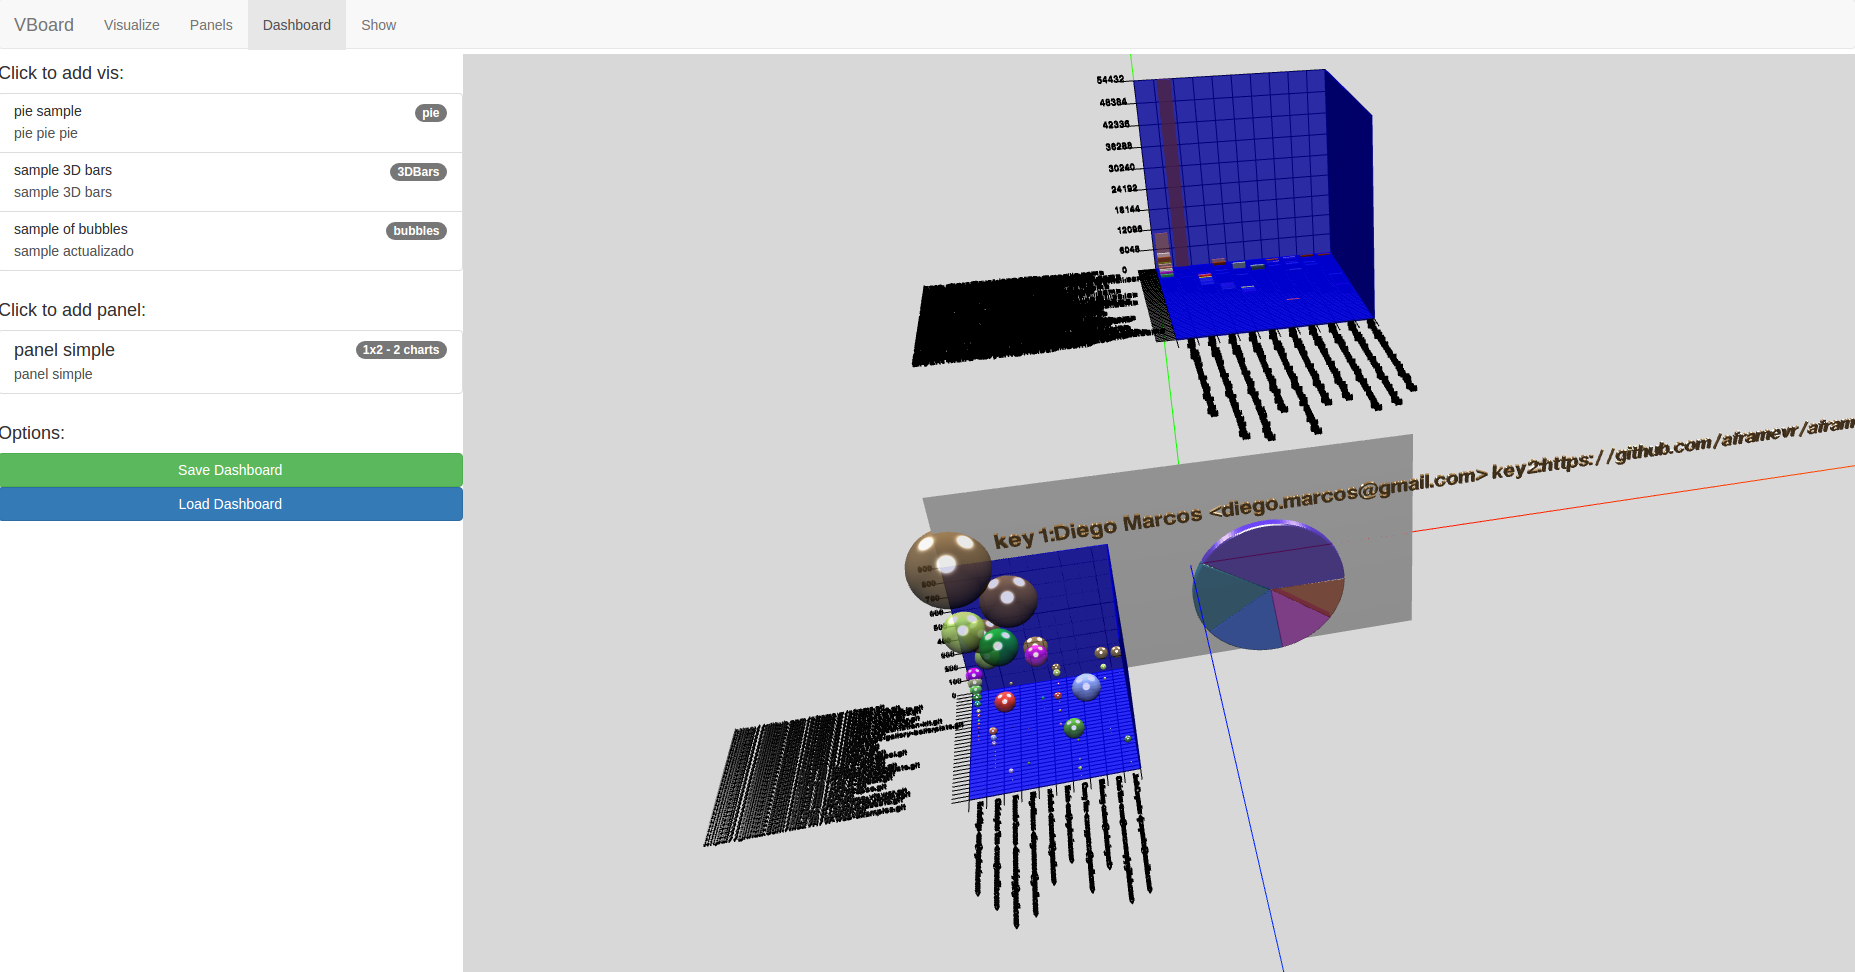
\includegraphics[width=16cm, keepaspectratio]{img/development/exampledashboard}
  \caption{Example of dashboard with one visualization and one panel inside}
  \label{fig:exampledashboard}
\end{figure}

\subsection{Show dashboard in stand alone version}

So that the user can visualize the dashboard in a simple way and also has no menu on the screen, (that is, that he/she only sees the 3D scene on the whole screen and can access the VR in a simple way, it will develop a new tab called "Show" that will show the list of saved dashboards, with the number of panels and charts it contains, and once it is clicked, the user will be redirected to a clean page where only the dashboard is located.

Therefore, the show tab will only have a content list:

\begin{figure}[H]
  \centering
  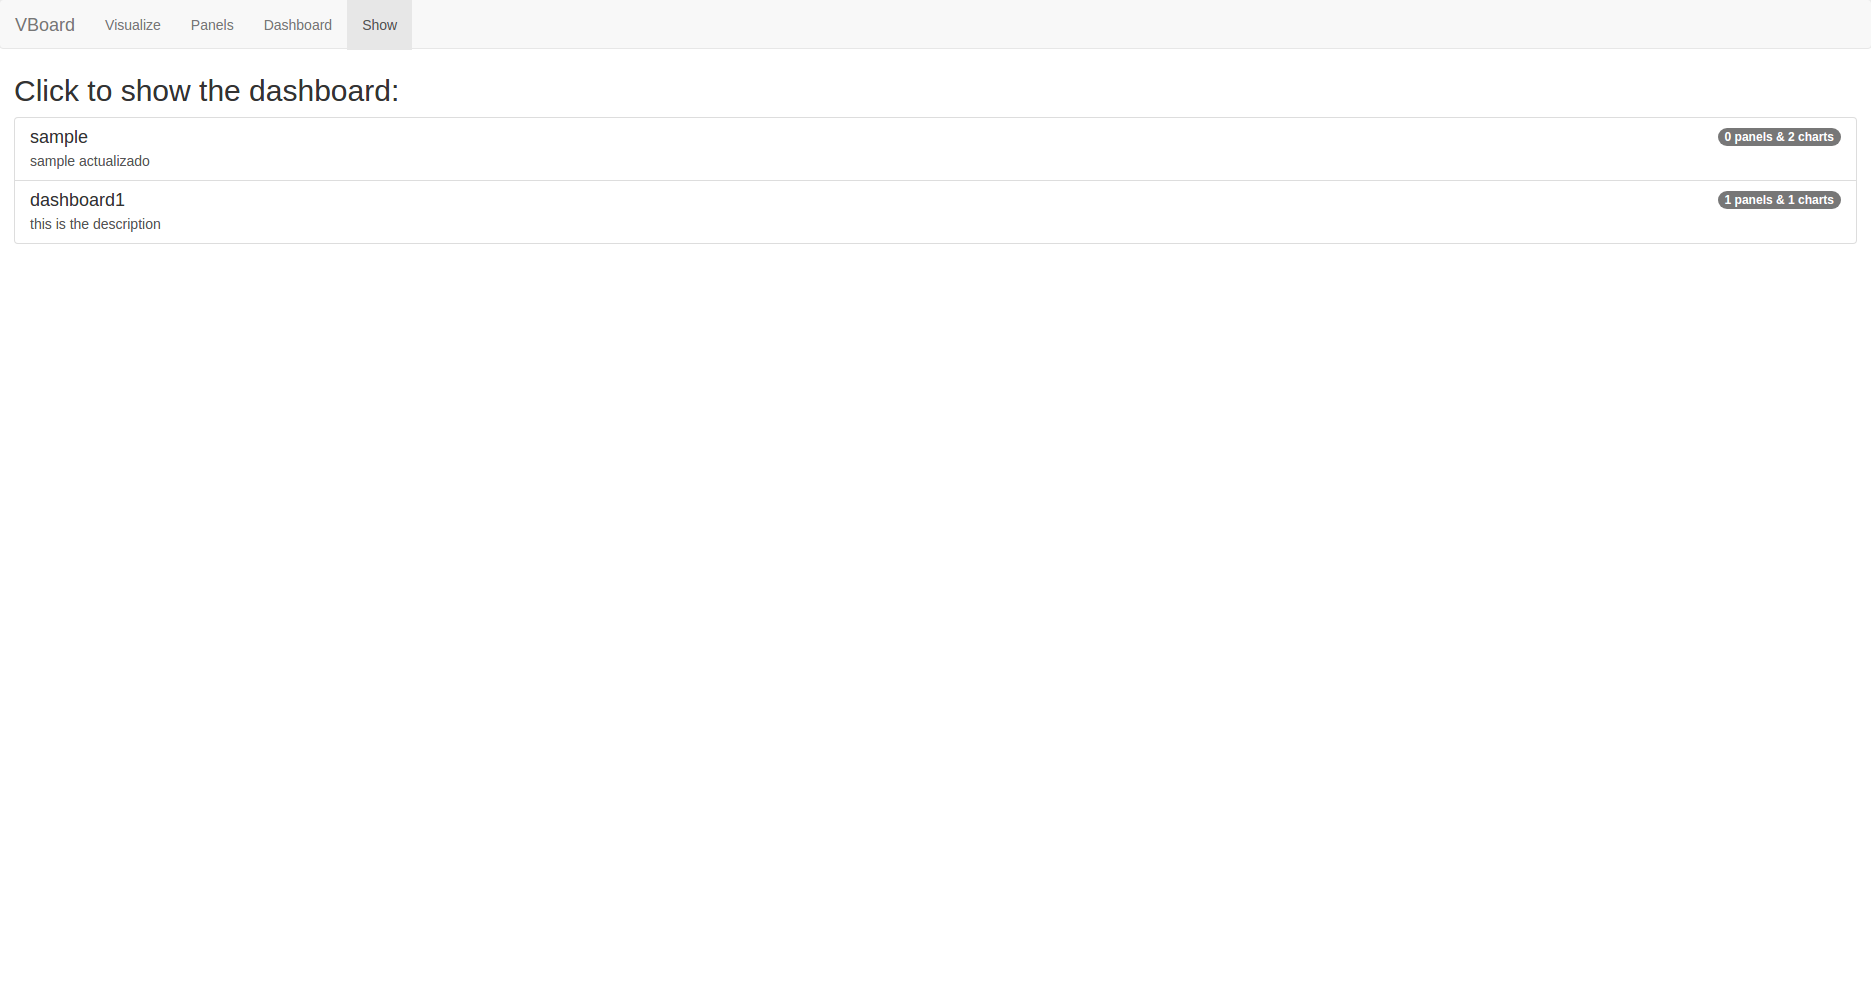
\includegraphics[width=16cm, keepaspectratio]{img/development/exampleshow}
  \caption{Example of the list in Show tab}
  \label{fig:exampleshow}
\end{figure}

And once the content is clicked, the user is redirected to a single url, so if the user only wants to access the dashboard in stand alone mode, he/she can access it with the url without going through the creation menus: \textit{localhost:8080/\#!/Show/dashboard\_name}

\begin{figure}[H]
  \centering
  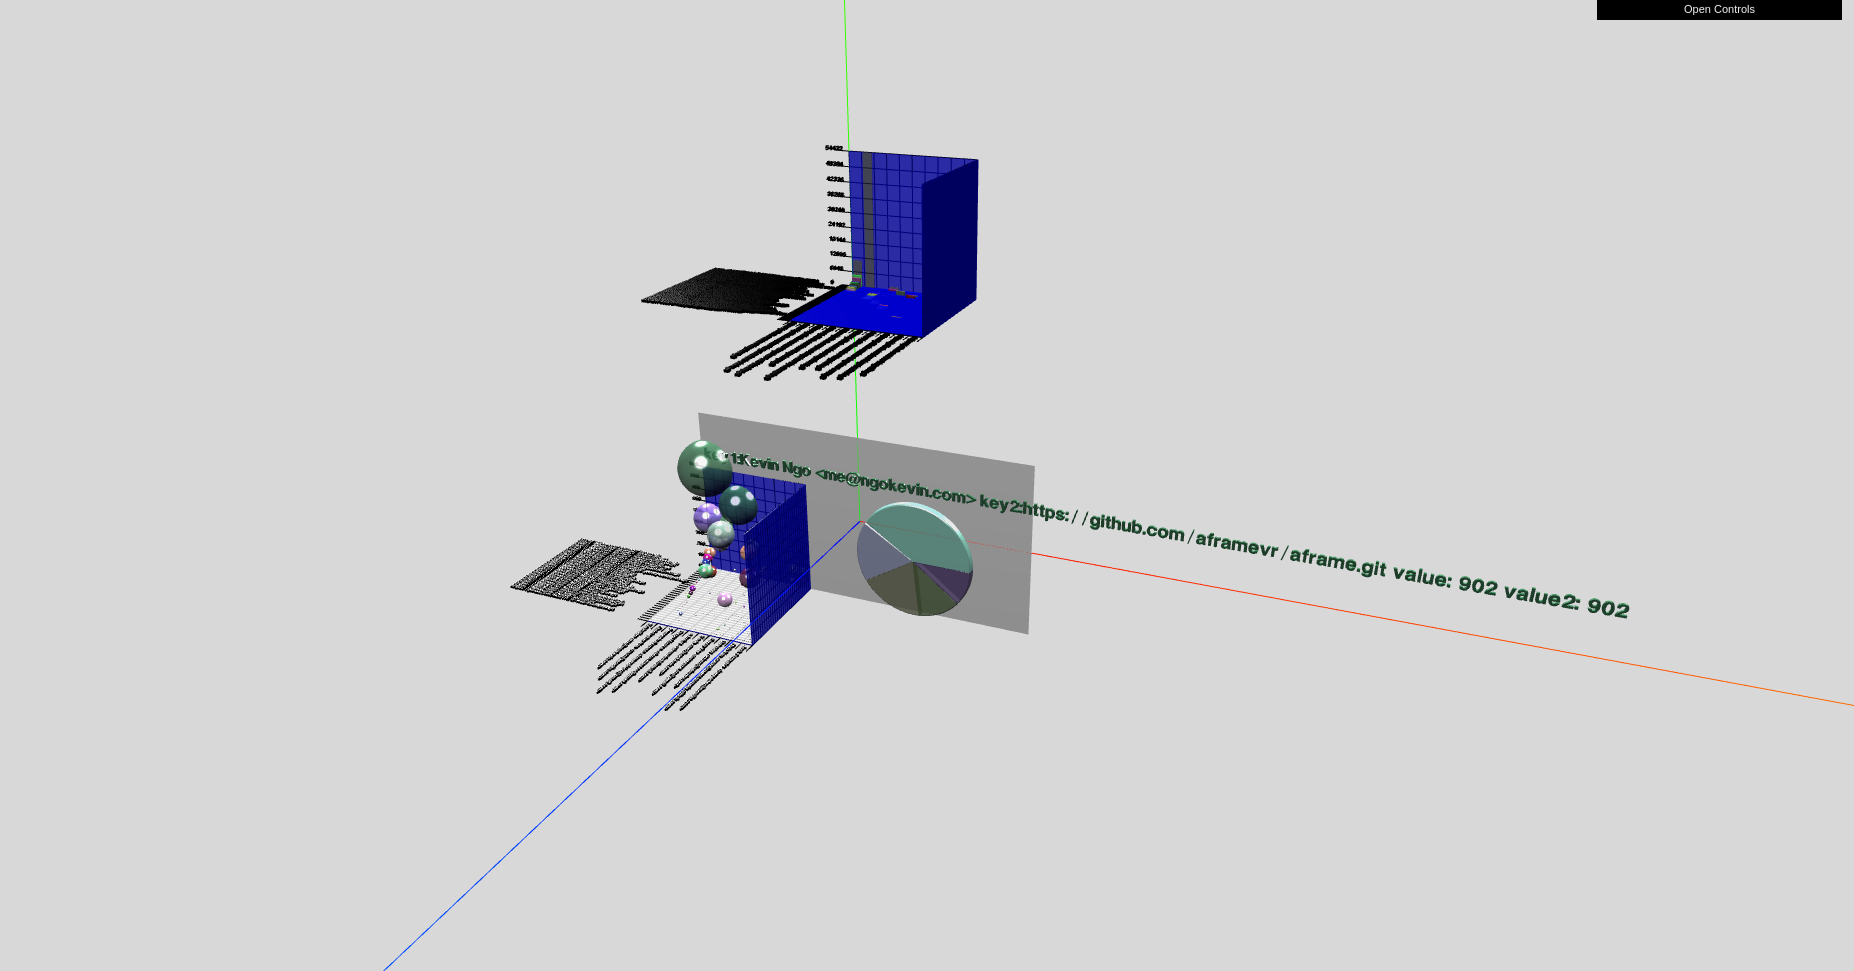
\includegraphics[width=16cm, keepaspectratio]{img/development/examplestandalone}
  \caption{Example of a Dashboard in stand alone mode}
  \label{fig:examplestandalone}
\end{figure}


The VBoard base application is complete, the next steps will be an improvement of it.

\section{Iteration 6: Integration with A-FrameDC}

In the middle of the development of the project, a former student of the university presented a JavaScript library for data visualization in 3D and VR, A-FrameDC\footnote{\url{https://fran-aguilar.github.io/a-framedc/}}, as well as ThreeDC but using A-Frame as a rendering engine (his degree thesis). From that moment, this project changed abruptly; we decided to include this new library, since A-Frame is a new library, that keeps developing, developed by a very important team in the community (Mozilla) and it is also open source. Therefore, this library would be included in VBoard, leading a parallel development of two versions, the version with ThreeDC and the version with A-FrameDC.

These two libraries barely have differences, both have the same methods to build 3D visualizations, but we must highlight the following differences that we find when including it:

\begin{itemize}
    \item A-FrameDC: when using A-Frame as a rendering engine, it includes the incorporation of VR natively, something that has not yet been developed by ThreeDC, so it would save us a lot of time for the implementation of Virtual Reality in the application.
    \item A-FrameDC: it does not have the functionality of "Panels", so it is impossible to build panels with this library. Likewise, the 3D panel concept does not make much sense, so this point would not be too negative.
    \item A-Frame: it does not have the development of 2D line visualization, but it has the visualization of smooth curve that is a curve.
\end{itemize}

After these pros and cons, the product owner and the development team decided that we would focus on this library as it is new and more powerful than ThreeDC.

\subsection{Modifications to VBoard}

As mentioned in the previous section, there is no need to make any significant changes to the application, since the methods of A-FrameDC and ThreeDC are the same, the only thing that had to be changed is the name of the object that returns the API to the instantiate (instantiate).

The next step is to eliminate the possibility of the section "Panels" of the application, for this the libraries genES and the front-end need to be modified to not save the panel logic in ElasticSearch and not to show the "Panels" tab in the application. Once the functionality is removed, the application would be as follows:

\begin{figure}[H]
  \centering
  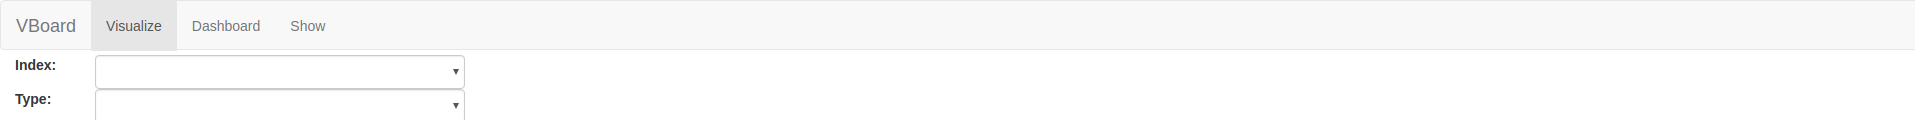
\includegraphics[width=16cm, keepaspectratio]{img/development/newnavbar}
  \caption{New navigation bar with A-FrameDC}
  \label{fig:examplestandalone}
\end{figure}

Besides, the most positive point of using A-FrameDC is the native incorporation of VR; in all the scenes created with A-Frame there is a button in the lower right corner that allows to activate this virtual reality.

\begin{figure}[H]
  \centering
  
\includegraphics[width=4cm, keepaspectratio]{img/development/vrbutton}
  \caption{VR button of A-frame}
  \label{fig:examplestandalone}
\end{figure}

The following images show some examples of construction of visualizations and dashboards with VBoard and this library:

\begin{figure}[H]
  \centering
  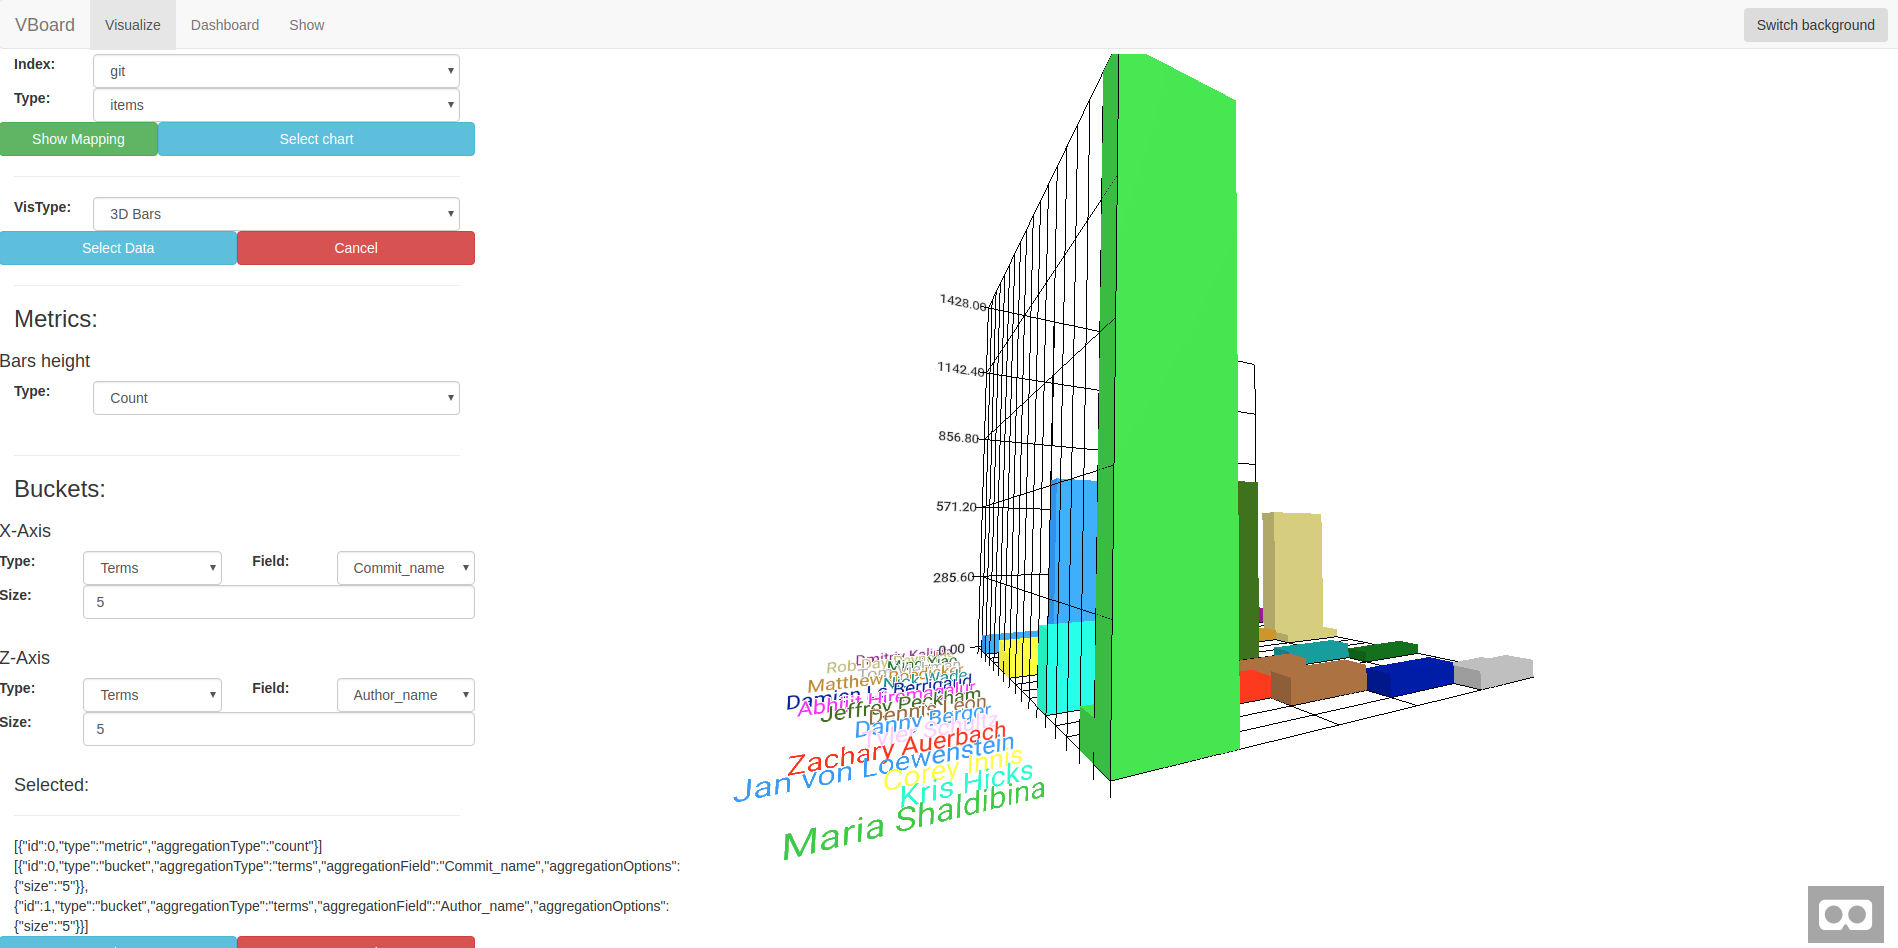
\includegraphics[width=16cm, keepaspectratio]{img/development/examplevisaframedc}
  \caption{Visualization example with A-FrameDC}
  \label{fig:examplestandalone}
\end{figure}

\begin{figure}[H]
  \centering
  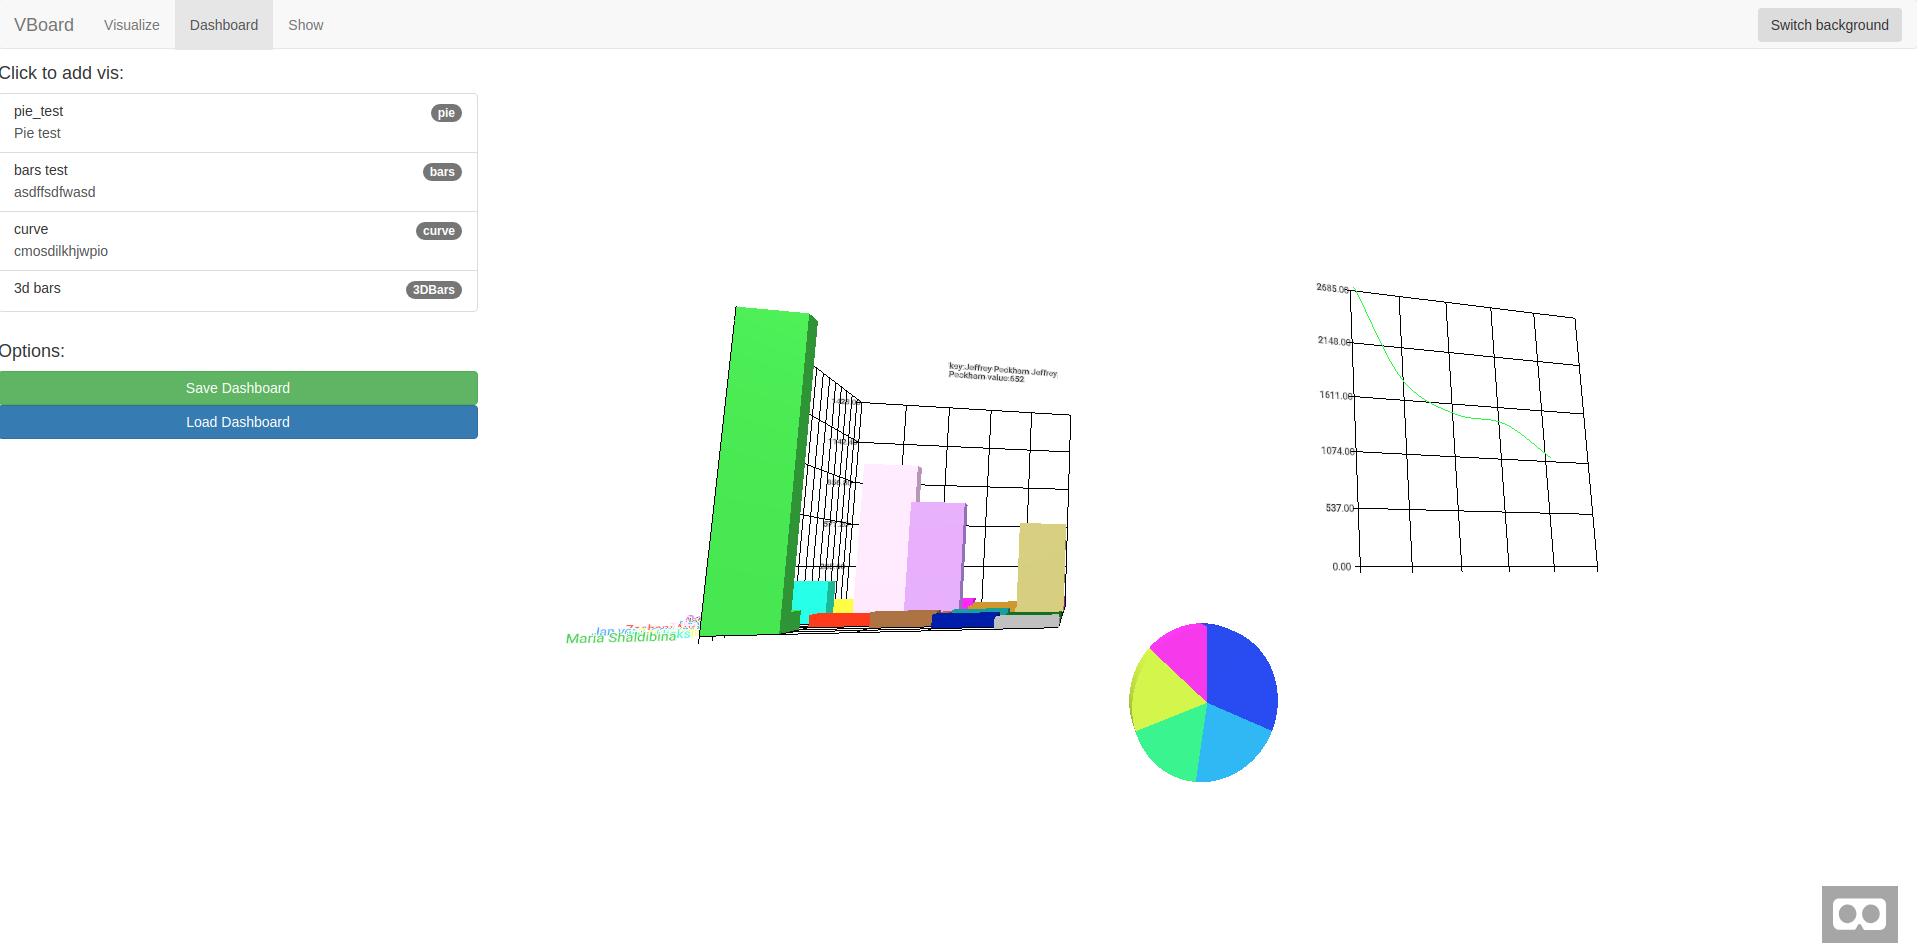
\includegraphics[width=16cm, keepaspectratio]{img/development/dashtestaframedc}
  \caption{Dashboard example with A-FrameDC}
  \label{fig:examplestandalone}
\end{figure}



\section{Iteration 7: Customization and optimization}

In order to make a clean and easily usable application, several customizations have been developed to improve it, as well as an optimization of the code to make it fast and scalable:

\begin{enumerate}
    \item Change background functionality
    \item Init process VBoard
    \item Rotation of the charts
    \item Information/Error messages when querying ElasticSearch
\end{enumerate}

\subsection{Change background functionality}

To see the dashboards in VR and in the "stand alone" mode, we implement an algorithm that changes between some wallpapers that are in the application, adding a button in the navigation bar to change it. These funds are limited and found in the application code:

\begin{figure}[H]
  \centering
  
\includegraphics[width=6cm, keepaspectratio]{img/development/switchbackgroundbutton}
  \caption{Switch background button in the navbar}
  \label{fig:examplestandalone}
\end{figure}


Once the dashboard is saved, the background it has assigned will be saved with it, so when it loads it will be loaded with it, the same happens when the stand alone mode and VR are loaded:

\begin{figure}[H]
 \centering
  \subfloat[In Dashboard tab]{
    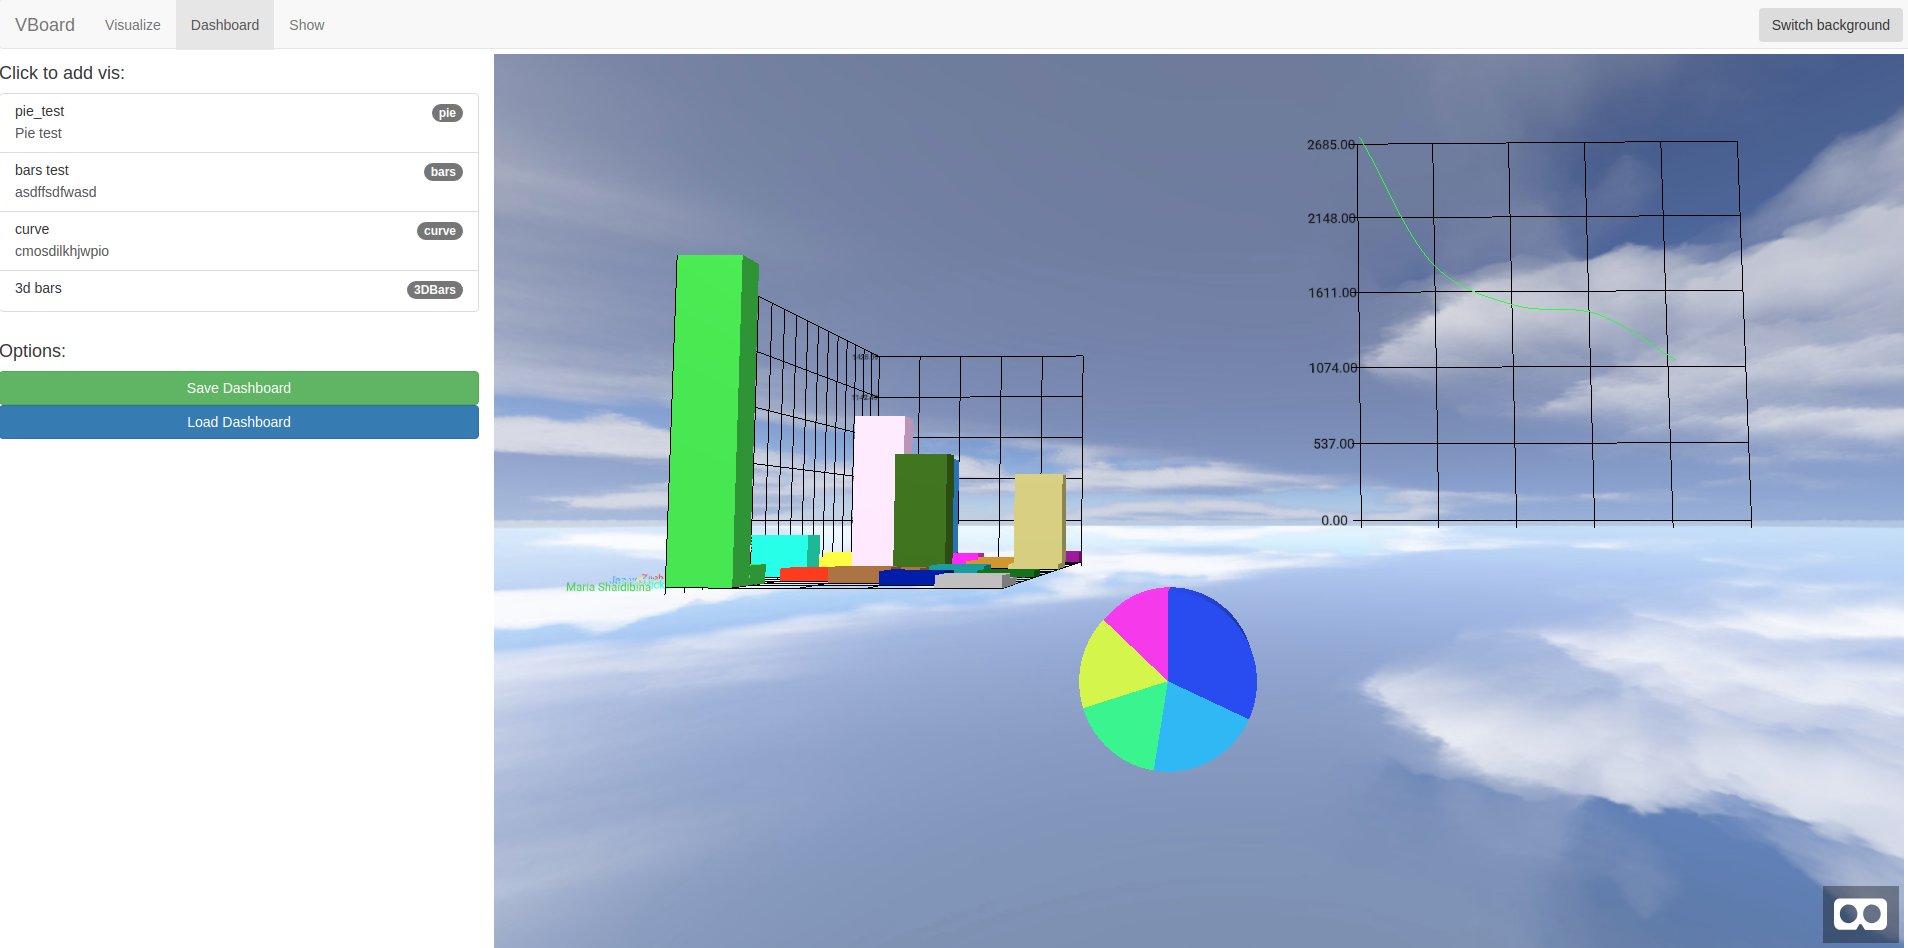
\includegraphics[width=0.5\textwidth]{img/development/backgroundaframedc}}
  \subfloat[In Show tab]{
    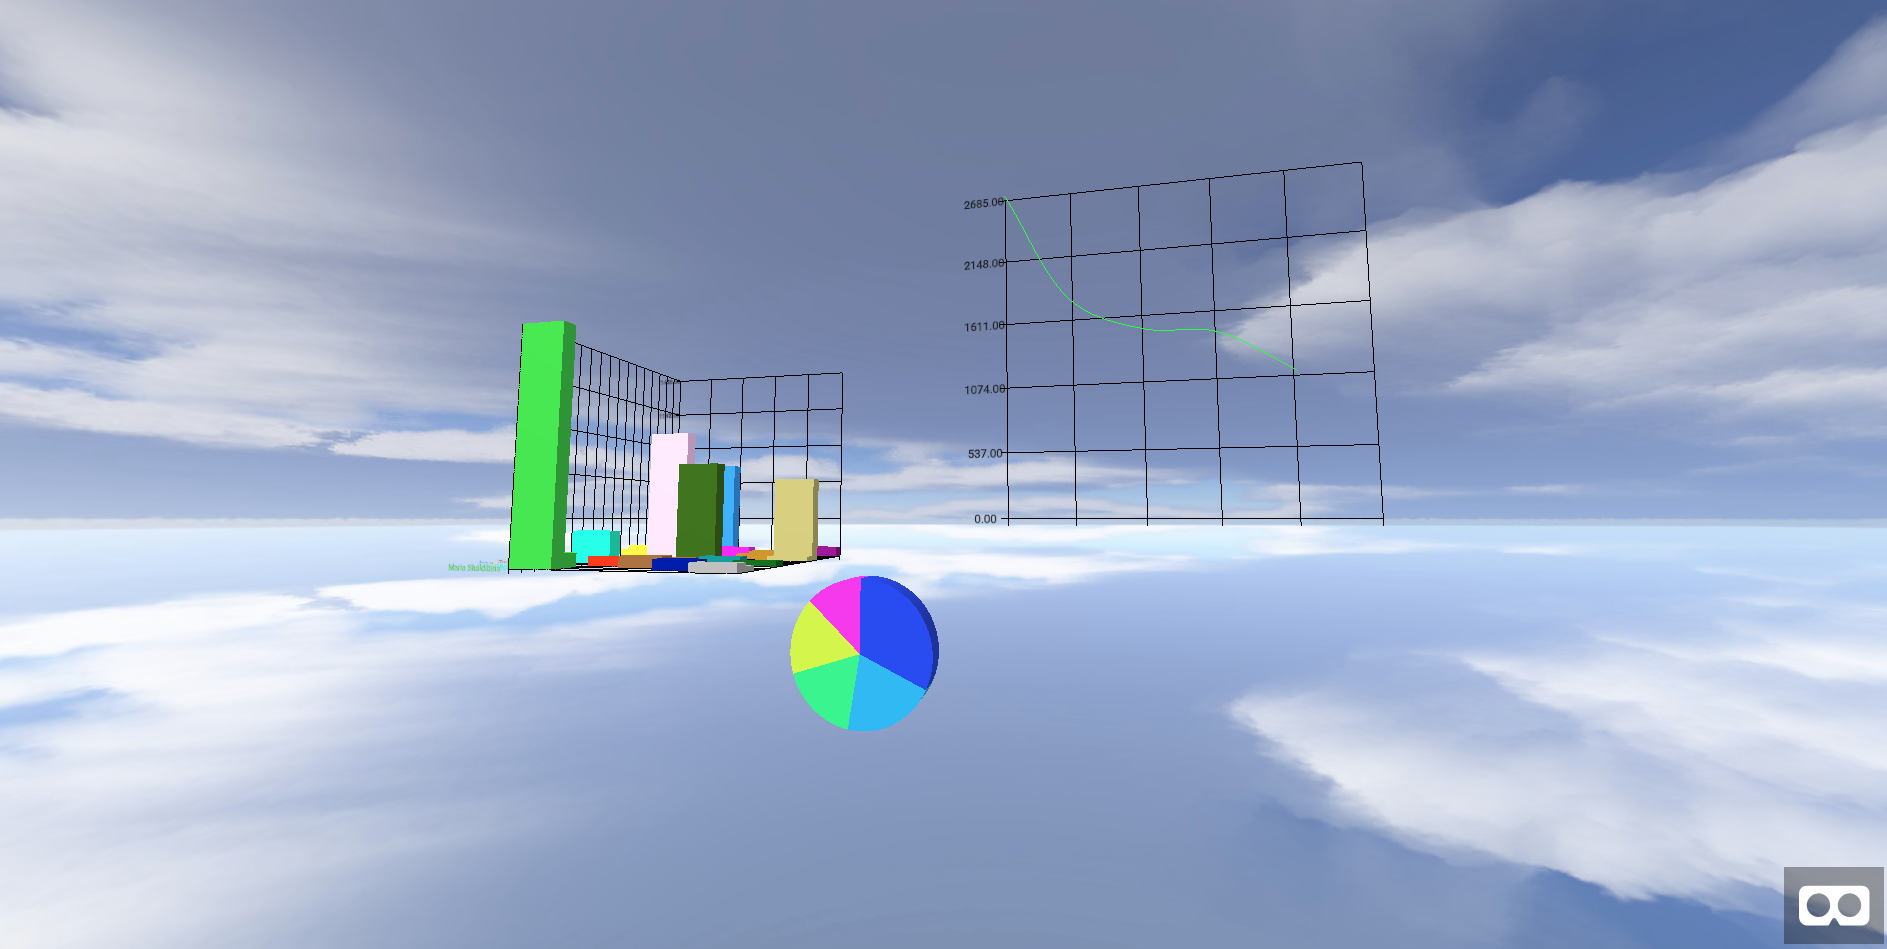
\includegraphics[width=0.5\textwidth]{img/development/showbackgroundaframedc}}
 \caption{Dashboard with background}
 \label{f:threedcexamples}
\end{figure}


This functionality has also been integrated into ThreeDC.



\subsection{Init process VBoard}

In order to create the index (index) of VBoard in ElasticSearch and verify that the application is well connected and has access to the index, we have developed a new phase to the application: the phase called Init, with its own AngularJS controller.

This phase verifies that you have access to the ElasticSearch defined in the Angular service within the application. If the connection is correct, it will try to access the index ".vboard"; if it can not find it, try to create it, making a PUT request with the mapping. If it is not correct, an error message will appear on the screen:

\begin{figure}[H]
  \centering
  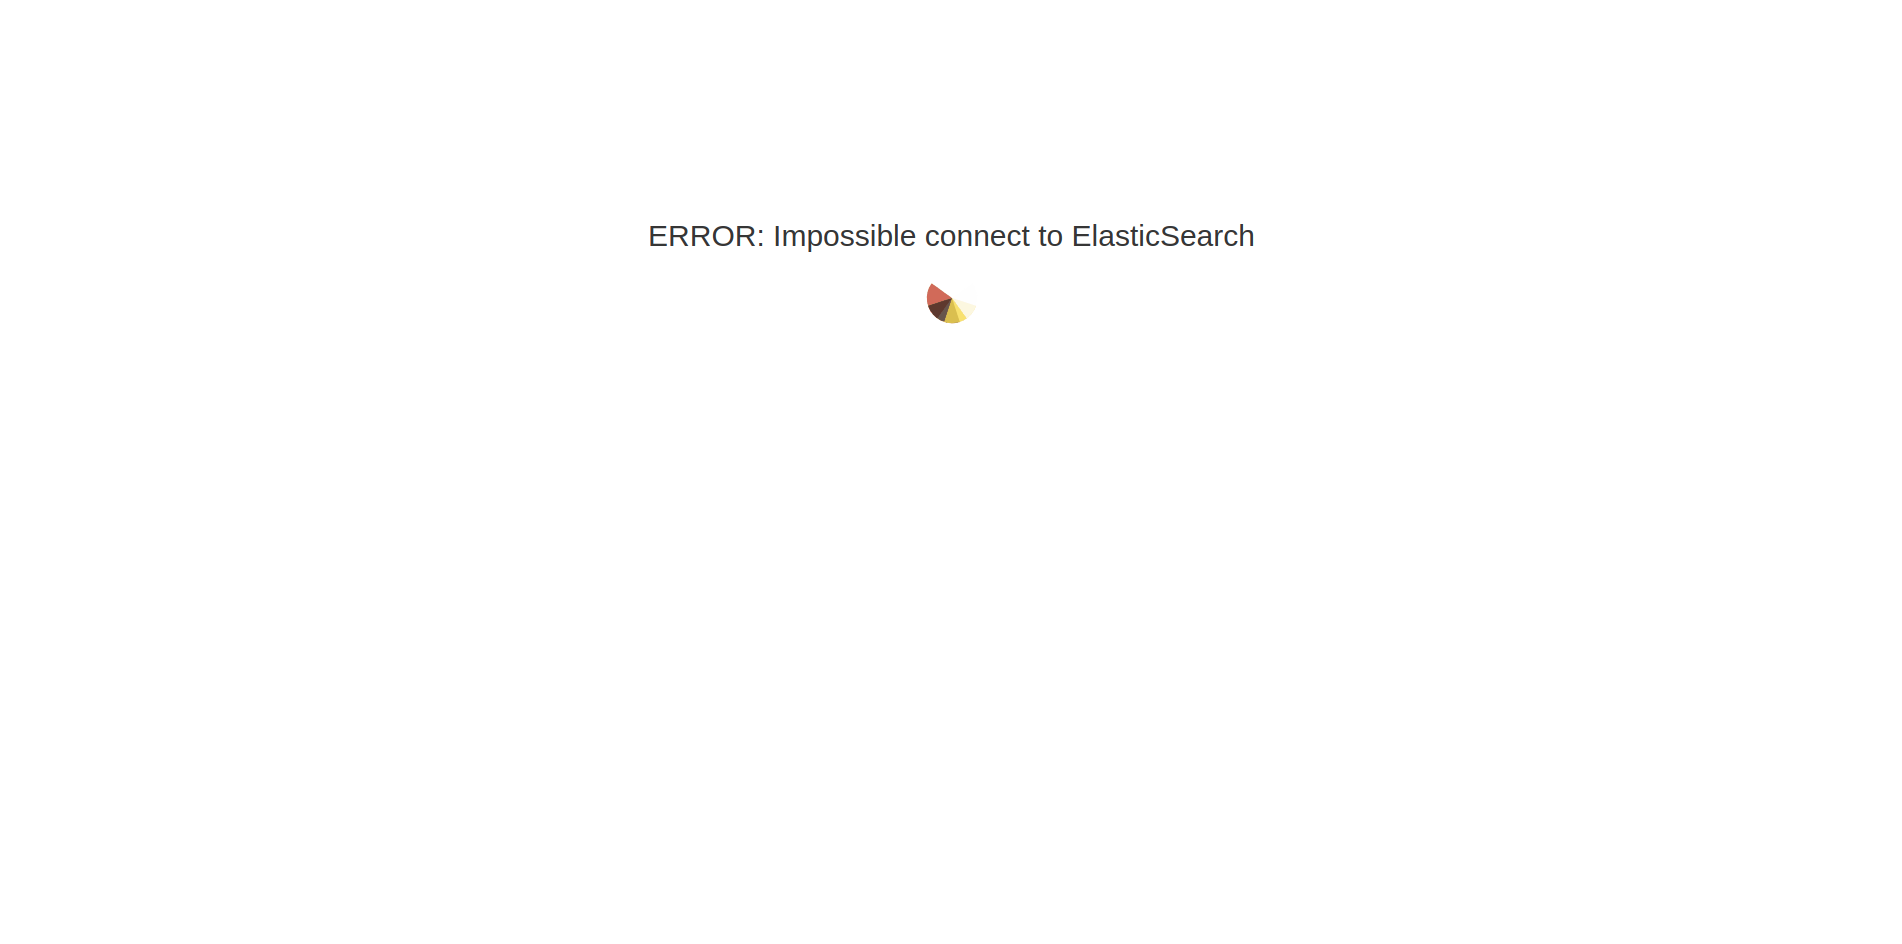
\includegraphics[width=16cm, keepaspectratio]{img/development/errorconnectes}
  \caption{Switch background button in the navbar}
  \label{fig:examplestandalone}
\end{figure}

In the event that you have been able to connect and have access to the ".vboard" index, a message will appear saying that everything went well, redirecting the user to the Visualize tab:

\begin{figure}[H]
  \centering
  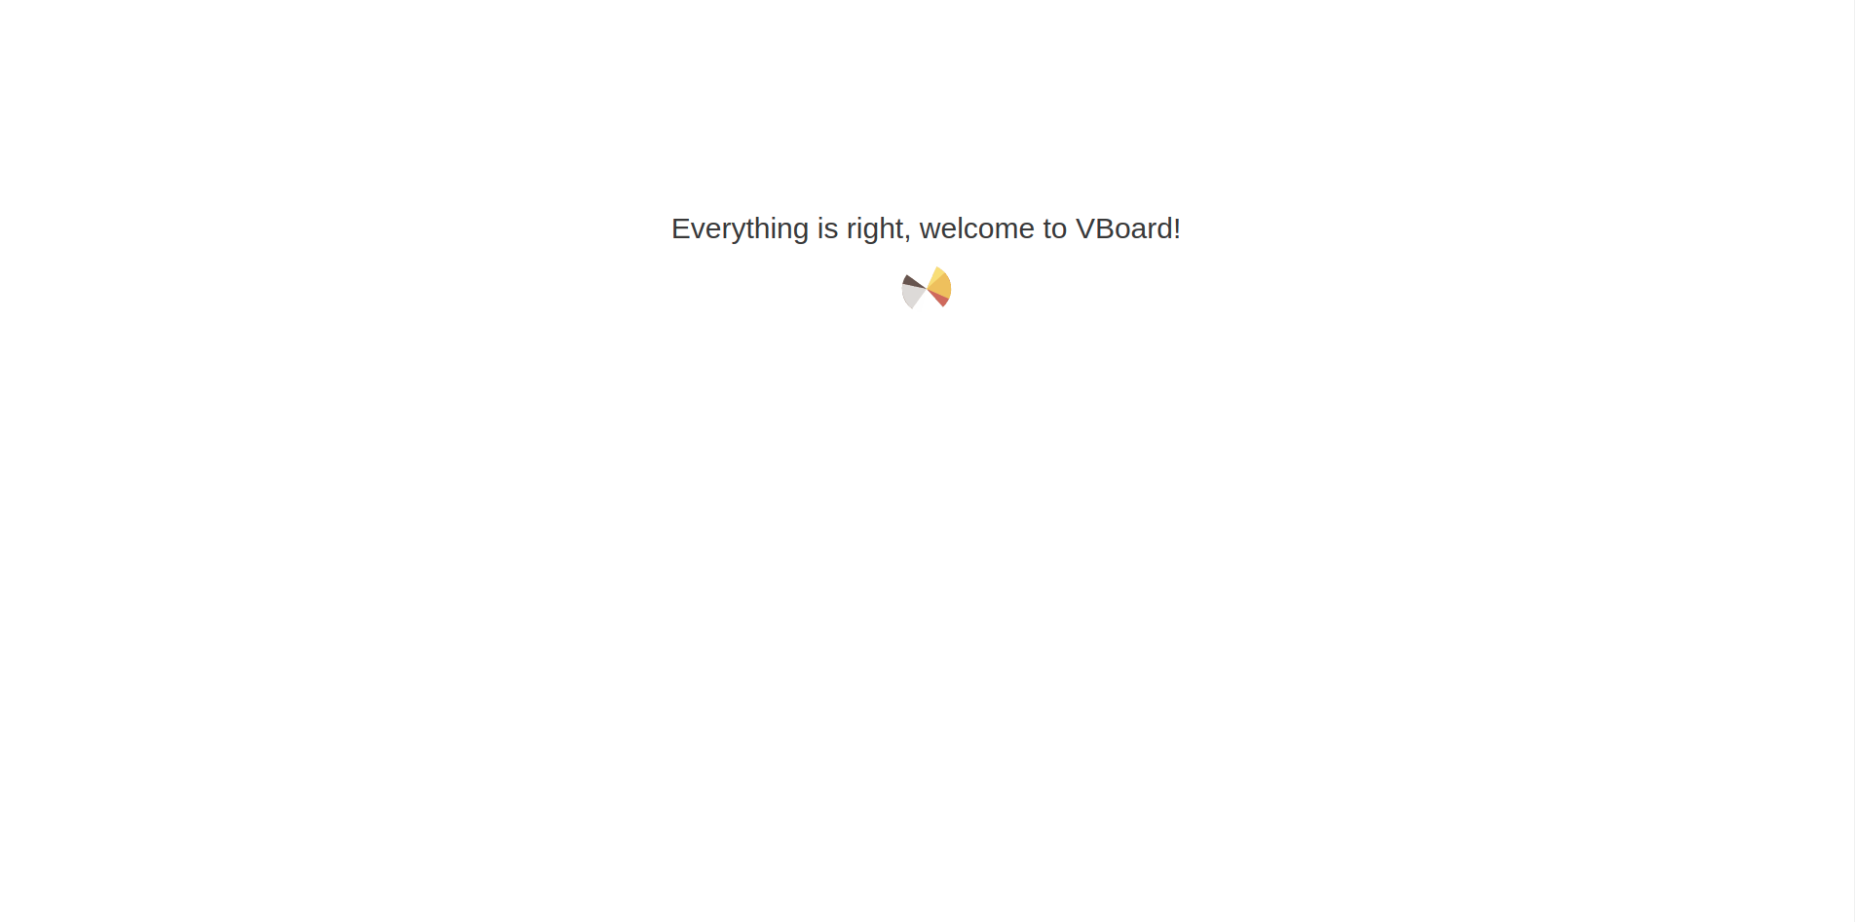
\includegraphics[width=16cm, keepaspectratio]{img/development/msgright}
  \caption{Switch background button in the navbar}
  \label{fig:examplestandalone}
\end{figure}

For all this functionality, more methods have been added to the genES library for all these requests. It must be checked that the connection with ElasticSearch is active, otherwise it will be redirected to the error screen shown above.

\subsection{Rotation of the charts}

It does not make sense to have a dashboard in 3D and VR and that you can not place the visualizations with a given rotation. Unfortunately, ThreeDC and A-frameDC do not support this option in their visualization construction method, so we have decided that we would develop that functionality ourselves by directly modifying the A-frameDC API.

The modification is simple because although the methods of the API do not allow it, there is that functionality below, directly in A-Frame. Therefore, once these methods have been modified, you have to add in the modal to add visualizations to a dashboard, 3 new inputs to define the rotation in 3 axes, "x", "y" and "z" (since we are in a 3D environment):

\begin{figure}[H]
  \centering
  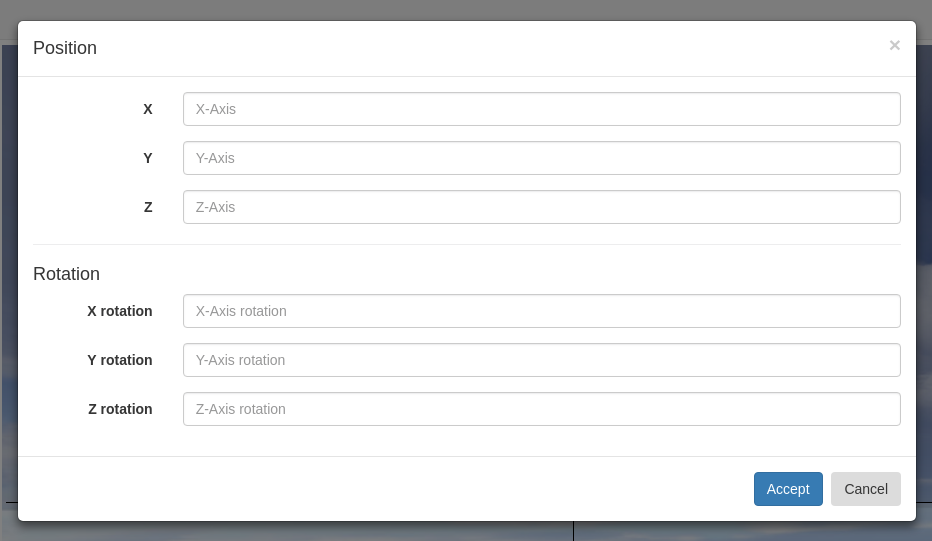
\includegraphics[width=16cm, keepaspectratio]{img/development/newformaframedc}
  \caption{Form now with rotation section}
  \label{fig:examplestandalone}
\end{figure}

With this functionality we can now put visualizations on the scene in a 360-degree range.

\subsection{Information/Error messages when querying ElasticSearch}

Another important improvement for the application is to notify the user when they access ElasticSearch to verify that the action was correct or erroneous. For this we have included the library "angular-ui-notification" to show through small modals in the upper right corner, error or success messages.

Thus, if the user was not able to access ElasticSearch to save/load an item, an error notification box would be displayed, and instead, if it could be accessed correctly, a green notification box will be displayed to show that everything is correct. The following screenshots show some examples of the use of these information tables:

\begin{figure}[H]
 \centering
  \subfloat[Error notification]{
    
\includegraphics[width=0.5\textwidth]{img/development/error_noti}}
  \subfloat[Success notification]{
    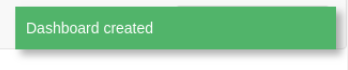
\includegraphics[width=0.5\textwidth]{img/development/success_noti}}
 \caption{Notifications}
 \label{f:threedcexamples}
\end{figure}


We understand that there is a lot of work ahead and that there are many improvements left, which will be discussed in the last chapter of the report detailing the future work on this application.

\section{Iteration 8: Dockerize application}
\label{sec:dockerize}

The last iteration, of great importance, has been to dock the application so that it can be deployed as a docker container in an easy and scalable way; this way, any person with basic knowledge of Docker can deploy VBoard in a simple way without having to follow many tedious installation steps.

To do this, 2 images of docker for VBoard have been created, one of them with the rendering engine ThreeDC and the other with A-FrameDC, being the A-FrameDC its main image. The first thing is to generate a Dockerfile defining the service of the application. In this case we have started with a "node-8" image since we use the node http server as server to deploy VBoard. The file Dockerfile is quite simple since all it does is clone the repo on a certain branch (to differentiate the version ThreeDC and A-FrameDC), install the npm dependencies (including the http server), expose port 8080 and define as "entrypoint" a script written in shell that configures the connection with ElasticSearch and starts the server:

\begin{lstlisting}[frame=single]
FROM node:8.12

MAINTAINER David Moreno Lumbreras "dmorenolumb@gmail.com"

RUN apt-get update -y

# Clone the repository
RUN git clone https://github.com/dlumbrer/VBoard -b integration-aframedc

# Install dependencies
WORKDIR VBoard
RUN npm install

# Install http-server
RUN npm install -g http-server

# Copy entrypoint
COPY docker-entrypoint.sh .
RUN chmod 755 docker-entrypoint.sh

# Expose port and init application
EXPOSE 8080
CMD ["./docker-entrypoint.sh"]
\end{lstlisting}

The docker-entrypoint is designed so that the IP of the ElasticSearch to which you want to connect VBoard (\textit{\$ELASTICSEARCH\_URL}) can be defined as an environment variable, and if this variable has not been defined, it will automatically connect to the ElasticSearch of the container host:

\begin{lstlisting}[frame=single]
#!/bin/bash

set -e

if [ "$ELASTICSEARCH_URL" != "" ]; then
        # If defined in the docker-compose
        sed -e "s|host: 'http://localhost:9200',$|host: '$ELASTICSEARCH_URL',|" -i /VBoard/app/service/ESService.js
else
        IP_HOST=$(/sbin/ip route|awk '/default/ { print $3 }')
        sed -e "s|host: 'http://localhost:9200',$|host: 'http://$IP_HOST:9200',|" -i /VBoard/app/service/ESService.js
fi

http-server
\end{lstlisting}

Once these images have been defined and tested, the next step is to host them in docker-hub, the place where docker images are stored so that anyone can access them through a tag. To do this, a link is made to the repository where the Dockerfile is located and image tags are defined that will be constructed from a branch or tag in the repository.

In the case of VBoard, the Dockerfile version of ThreeDC and A-FrameDC are in the "docker" branch, so we configure the construction of images as follows:

\begin{figure}[H]
  \centering
  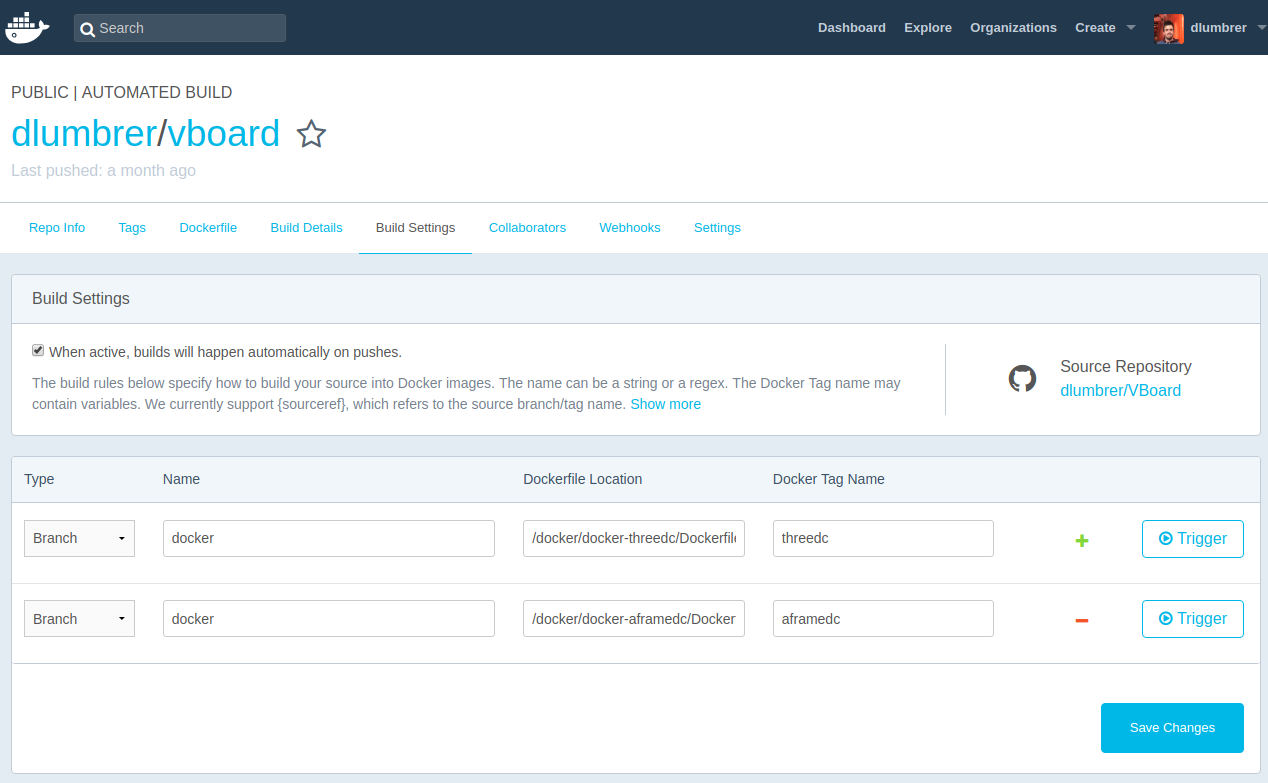
\includegraphics[width=16cm, keepaspectratio]{img/development/docker-hub-0}
  \caption{Build Settings for VBoard}
  \label{fig:examplestandalone}
\end{figure}

So we will have two available VBoard images, each with a different tag:

\begin{figure}[H]
  \centering
  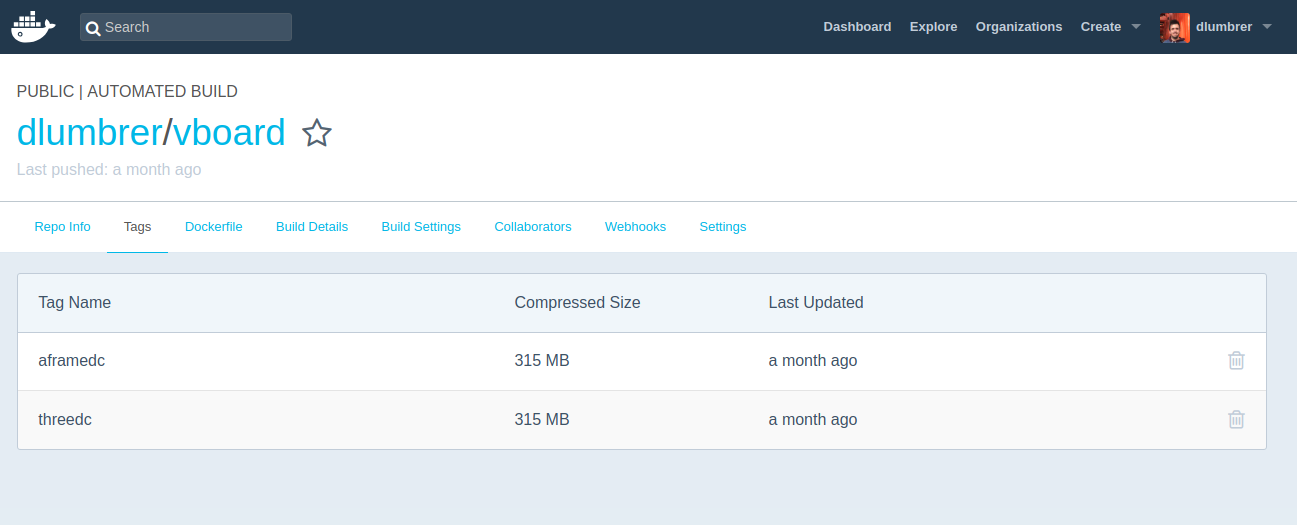
\includegraphics[width=16cm, keepaspectratio]{img/development/dockerhub}
  \caption{Image tags for VBoard}
  \label{fig:examplestandalone}
\end{figure}

With the images built, we can download them and launch containers from them simply by displaying the tags \textit{dlumbrer/VBoard:aframedc} and \textit{dlumbrer/VBoard:threedc}.

 
%%%%%%%%%%%%%%%%%%%%%%%%%%%%%%%%%%%%%%%%%%%%%%%%%%%%%%%%%%%%%%%%%%%%%%%%%%%%%%%%
%%%%%%%%%%%%%%%%%%%%%%%%%%%%%%%%%%%%%%%%%%%%%%%%%%%%%%%%%%%%%%%%%%%%%%%%%%%%%%%%
% RESULTADOS %
%%%%%%%%%%%%%%%%%%%%%%%%%%%%%%%%%%%%%%%%%%%%%%%%%%%%%%%%%%%%%%%%%%%%%%%%%%%%%%%%
\cleardoublepage
\chapter{Design and results}
\label{chap:dai}

\section{Introduction}
\label{sec:dint}

In this chapter we will describe the aspects of the final application. We will start defining its structure, in code and in visualization. Then, we will explain its functioning next to a user's guide in order to define de different types of visualization and dashboard that the application has. Finally, we will test the application with data offered by the product owner.

\section{Structure}

As we've already explained in section \ref{sec:it1}, to develop a front-end application in AngularJS, it has been followed a standard file structure of this framework. According to this model, VBoard has the following file structure:

\begin{figure}[H]
  \centering
  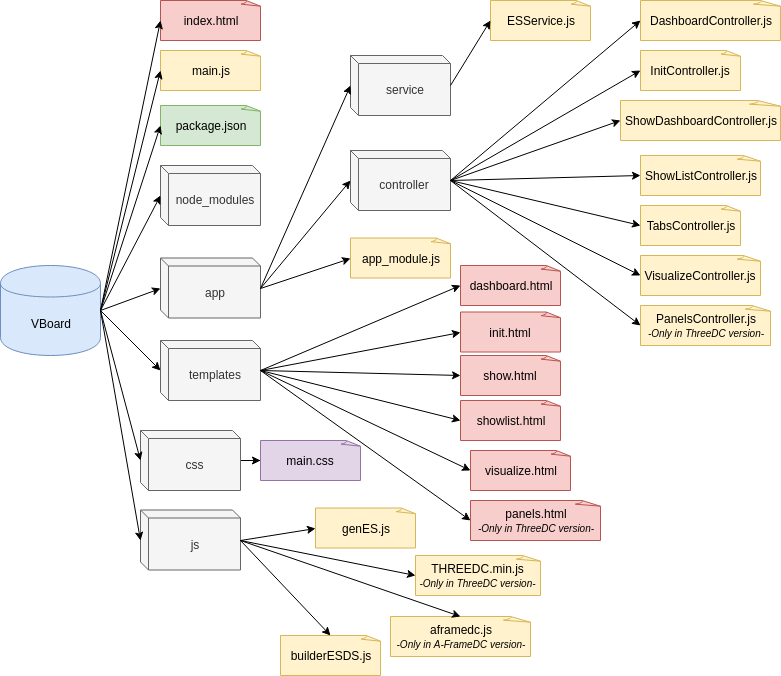
\includegraphics[width=16cm, keepaspectratio]{TFM/img/results/Vboard.png}
  \caption{Diagram of the files}
  \label{fig:codediagram}
\end{figure}

The yellow files correspond to JavaScript codes, red ones to HTML, purple ones to CSS and the green ones to JSON files.

Specifically:
\begin{itemize}
    \item File \textit{index.html}: basic html file where the external libraries are loaded (CDN or in local) and where the navigation bar of VBoard is defined.
    \item File \textit{main.js}: file where the AngularJS application is defined, in this case VBoard.
    \item File \textit{package.json}: file where the metadata of VBoard, as well as the necessary dependencies npm to is later installation are located.
    \item Folder \textit{node\_modules}: place where the dependencies npm will be installed.
     \item Folder \textit{app}: inside this folder the “core” of the JavaScript application is located; within it are the following folders: 
    \begin{itemize}
        \item Folder \textit{service}: folder where the AngularJS services are to be used in VBoard, in this case there is only one, with the name of \textit{ESService.js}, where the ElasticSearch client to be used in VBoard is defined.
        \item Folder \textit{controller}:  inside this folder are all the controllers of the different zones of VBoard, there is the controller of all the logic of the navigation bar in the file \textit{TabsController.js}, the logic of the process of starting VBoard in the file \textit{InitController.js}, the logic of each of the available tabs "Visualize, Panels, Dashboard and Show" is its corresponding files.
        \item File \textit{app\_module.js}: File where the VBoard application is instantiated, where all the controllers, templates and files of the AngularJS framework you need are defined.
    \end{itemize}
    \item Folder \textit{templates}: Inside this folder there are the 5 html codes corresponding to the 5 zones that require HTML that are inside VBoard, Init, Visualize, Panels, Dashboard and Show.
    \item Folder \textit{css}: In this folder there are the CSS codes, in this case there is only one since the CSS used is very few and therefore is a great point to improve in VBoard.
    \item Folder \textit{js}: This folder contains the JavaScript libraries that have not been installed by npm, that is, in this case, the genES and builderESDS that have been developed by us, and the 3D rendering libraries, \textit{aframedc.js} and \textit{THREEDC.min.js}.
\end{itemize}

The visual structure is also defined in the section \ref{sec:it1}, so it will not be detailed again; in the following sections we will explain a user guide and some examples where everything will be clear.


\section{Installation steps}
There are few ways to install VBoard, from the source code in the repository, from the releases, or from the docker image that is in dockerhub. All these installation steps are included in the README.md\footnote{\url{https://github.com/dlumbrer/VBoard}} of the repository.

\subsection{From repository}
Directly installation from the source code, the steps are:
\begin{enumerate}
    \item Clone the repository, choosing a different branch in order to change between ThreeDC and A-FrameDC
    \begin{itemize}
        \item For A-FrameDC version: \textit{git clone https://github.com/dlumbrer/VBoard -b integration-aframedc}
        \item For ThreeDC version: \textit{git clone https://github.com/dlumbrer/VBoard -b integration-threedc}
    \end{itemize}
    \item Change directory: \textit{cd VBoard}
    \item Install npm dependencies, it is necessary to have installed node: \textit{npm install}
    \item (Optional) Install node http-server: \textit{npm install -g http-server}
    \item Run VBoard server: \textit{http-server}
\end{enumerate}

The fifth step is optional because you can use any server of http, for instance the http simple server from python.

\subsection{From releases}
This is the easiest way to launch VBoard if don't want to install it via source code or docker. It is so simple that you have to download the zip/tar binaries of the selected version (ThreeDC or A-FrameDC) from the GitHub VBoard releases page \footnote{\url{https://github.com/dlumbrer/VBoard/releases}}, go inside the uncompressed folder and launch it with your favourite http-server (I recommend the http-server from node).

\subsection{Docker}
As we explained in section \ref{sec:dockerize}, there are docker images of the two versions of VBoard. The information about the images are inside the "docker" branch of the repository\footnote{\url{https://github.com/dlumbrer/VBoard/tree/docker}}, also, there are inside a few examples of how to deploy VBoard using docker-compose.

If we want to deploy VBoard, we can do it easily with docker launching a container in one line, but the easiest and useful way is to use docker-compose. There are two ways to deploy VBoard with docker-compose, one with ElasticSearch included or one just with VBoard:

\begin{itemize}
    \item \textbf{A-FrameDC or ThreeDC + ElasticSearch}: If you want a full installation with the A-FrameDC or ThreeDC version and a ElasticSearch, I recommend to use this docker-compose:
    \begin{lstlisting}[frame=single]
    ElasticSearch:
      image: docker.elastic.co/ElasticSearch/ElasticSearch:5.6.0
      ports:
        - "9200:9200"
      volumes:
        - ./config/ElasticSearch.yml:/usr/share/ElasticSearch/config/ElasticSearch.yml:ro
      environment:
        - ES_JAVA_OPTS=-Xms2g -Xmx2g
        - transport.host=127.0.0.1
        - xpack.security.enabled=false
    
    vboard:
      image: dlumbrer/vboard:aframedc
      # image: dlumbrer/vboard:threedc # Uncomment this line if you want the ThreeDC version
      ports:
        - "8080:8080"
    \end{lstlisting}
    Note that the VBoard app will be connected to ElasticSearch automatically.
    
    \item \textbf{A-FrameDC or ThreeDC without ElasticSearch}: This compose will deploy just VBoard:
    \begin{lstlisting}[frame=single]
    vboard:
      image: dlumbrer/vboard:aframedc
      # image: dlumbrer/vboard:threedc # Uncomment this line if you want the ThreeDC version
      ports:
        - "8080:8080"
      environment:
        - ELASTICSEARCH_URL=http://localhost:9200
    \end{lstlisting}
    \textbf{Important}: You have to modify the environment variable "ELASTICSEARCH\_URL" to you ElasticSearch url.
    
    \item Moreover, we offer a docker-compose file in order to deploy just ElasticSearch, for instance if you want an ElasticSearch in one machine and VBoard in other, or you want to install VBoard from releases or source code but you want to use ElasticSearch in a docker container:
    \begin{lstlisting}[frame=single]
    ElasticSearch:
      image: docker.elastic.co/ElasticSearch/ElasticSearch:5.6.0
      ports:
        - "9200:9200"
      volumes:
        - ./config/ElasticSearch.yml:/usr/share/ElasticSearch/config/ElasticSearch.yml:ro
      environment:
        - ES_JAVA_OPTS=-Xms2g -Xmx2g
        - transport.host=127.0.0.1
        - xpack.security.enabled=false
    \end{lstlisting}
    
In order to deploy VBoard with docker, it is needed a few acknowledge of Docker.




\end{itemize}

\section{User Guide}

Later, we will define a user guide, explaining step by step how to init VBoard, how to produce visualizations, how to save it, how to produce dashboards and how to save it and see it in the stand-alone version.  As the menu and the process is the same, we will explain the user guide for the A-FrameDC version, focusing in examples and how to take advantage of all functionality of VBoard. So we explain how to produce an entire dashboard with visualizations from scratch:

\subsection{Init VBoard}

First of all, VBoard will check its connection to ElasticSearch, these are the steps that will be seen when entering the application:

\begin{enumerate}

    \item First, VBoard will notify the user who is making configurations:
    \begin{figure}[H]
      \centering
      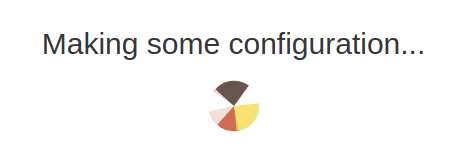
\includegraphics[width=8cm, keepaspectratio]{img/results/Init1}
      \caption{First info message from VBoard}
      \label{fig:onlynodes}
    \end{figure}
    When it cannot connect to ElasticSearch, this error message will appear:
    \begin{figure}[H]
      \centering
      
\includegraphics[width=11cm, keepaspectratio]{img/results/Init2}
      \caption{Error connecting to ElasticSearch}
      \label{fig:onlynodes}
    \end{figure}
    \item Once connected to ElasticSearch, it will search the index \textit{.vboard}, and then there are two options:
    \begin{itemize}
        \item The index doesn't exist, so it will try to create it, showing this information message:
        \begin{figure}[H]
          \centering
          \includegraphics[width=9cm, keepaspectratio]{img/results/Init3}
          \caption{Creating .vboard index}
          \label{fig:onlynodes}
        \end{figure}
        To do this, the mapping of the index will be uploaded. In the case that it could not upload the mapping for any reason, the following error message will be displayed:
        \begin{figure}[H]
          \centering
          \includegraphics[width=9cm, keepaspectratio]{img/results/Init4}
          \caption{Unexpected error}
          \label{fig:onlynodes}
        \end{figure}
        If it has successfully uploaded the mapping, there will be a notification saying that everything is fine and it will enter VBoard:
        \begin{figure}[H]
          \centering
          \includegraphics[width=11cm, keepaspectratio]{img/results/Init5}
          \caption{Index and mapping created}
          \label{fig:onlynodes}
        \end{figure}
        \item The index is already created and therefore, everything is ready; this information message will appear:
        \begin{figure}[H]
          \centering
          \includegraphics[width=9cm, keepaspectratio]{img/results/Init6}
          \caption{Everything right}
          \label{fig:onlynodes}
        \end{figure}
    \end{itemize}
\end{enumerate}

Finally, if everything is well loaded, VBoard will redirect you to the Visualize tab.

\subsection{Visualize}

In order to build a 3D visualization, go to the tab "Visualize" and follow these steps:
\begin{enumerate}
    \item Select the index and the type of your ElasticSearch where the data is going to be visualized, then click on "Select chart" button:
    \begin{figure}[H]
      \centering
      \includegraphics[width=8cm, keepaspectratio]{img/results/selectindex}
      \caption{Index and type selection}
      \label{fig:onlynodes}
    \end{figure}
    Note that there are another button call "Show mapping", it is explained at the end of this section, in the Options section.
    \item Select chart type: Pie, Bars, Smooth Curve, 3D Bars and Bubbles
    \begin{figure}[H]
      \centering
      \includegraphics[width=8cm, keepaspectratio]{img/results/selectvistype}
      \caption{Chart selection}
      \label{fig:onlynodes}
    \end{figure}
    \item Select the aggregation data that you want to visualize. Note that each chart could require more or less aggregations (metrics/buckets).
    \begin{figure}[H]
      \centering
      \includegraphics[width=8cm, keepaspectratio]{img/results/selectdata}
      \caption{Data selection}
      \label{fig:onlynodes}
    \end{figure}
    \item Click on Play in order to see the visualization or Cancel if you want to go back. Later we will show two examples of visualizations
\end{enumerate}


Moreover there are a few options apart from the build visualization process:
\begin{enumerate}
    \item Show mapping button, this button will show the mapping of the index selected, the mapping will be showed at the end of the page in a JSON format:
    \begin{figure}[H]
      \centering
      \includegraphics[width=16cm, keepaspectratio]{img/results/examplemapping}
      \caption{Show mapping result at the end of the page}
      \label{fig:onlynodes}
    \end{figure}
    \item Show Response (JSON), this button will show the result of the query of the aggregation selected before, in a JSON format at the end of the page. It will be two columns, one representing the data in raw and the other the aggregated data:
    \begin{figure}[H]
      \centering
      \includegraphics[width=16cm, keepaspectratio]{img/results/exampleresponse}
      \caption{Show response example}
      \label{fig:onlynodes}
    \end{figure}
    \item Save visualization, this button will open a modal with a form in order to save the current visualization, the form contains a name and a description that will be saved with the visualization:
    \begin{figure}[H]
      \centering
      \includegraphics[width=16cm, keepaspectratio]{img/results/examplesave}
      \caption{Example save modal}
      \label{fig:onlynodes}
    \end{figure}
   \item Load visualization, this button will open a modal with a list of the saved visualization, each item is a button that will load the visualization in the current page. Each item shows the title, the description and the type of the saved visualization:
    \begin{figure}[H]
      \centering
      \includegraphics[width=16cm, keepaspectratio]{img/results/exampleload}
      \caption{Example load modal}
      \label{fig:onlynodes}
    \end{figure}
    \item Switch background, this button switches the current background in order to see the visualization in different environments, the background is just to show the aspect, it will not save it with the visualization.
\end{enumerate}

Now, we are ready to build, save and load visualizations.

\subsubsection{Examples}

To finish, these are two examples of visualizations that you can build with VBoard:

\begin{figure}[H]
 \centering
  \subfloat[3D Bars chart]{
    \includegraphics[width=0.5\textwidth]{img/results/examplevis1}}
  \subfloat[Pie Chart]{
    \includegraphics[width=0.5\textwidth]{img/results/examplevis2}}
 \caption{Example charts built with A-FrameDC in VBoard}
 \label{f:threedcexamples}
\end{figure}

\subsection{Panels - Only in ThreeDC version}
In order to build a Panel, a flat plane with visualization, you have to have installed the ThreeDC version, then go to the Panels tab. By default, you will see a default panel with 3 rows, 3 columns, [500,500] of dimension and 0.6 of opacity. Then, let's fill the panel with visualization, you will see a list of the saved visualization on the left control menu:
\begin{enumerate}
    \item Click on one of the available visualizations and a modal will appear in order to define in which row and column you want to put the visualization:
    \begin{figure}[H]
      \centering
      \includegraphics[width=16cm, keepaspectratio]{TFM/img/results/exampleaddvistopanel.png}
      \caption{Modal add chart to a panel}
      \label{fig:onlynodes}
    \end{figure}
    \item Once a visualization has been added to the panel, you will see the panel with the visualization:
    \begin{figure}[H]
      \centering
      \includegraphics[width=16cm, keepaspectratio]{TFM/img/results/examplepanelbubbles.png}
      \caption{Panel with one chart}
      \label{fig:onlynodes}
    \end{figure}
\end{enumerate}

Moreover there are a few options apart from the build panel process:
\begin{enumerate}
    \item New Panel button, this button opens a modal with a form in order to reset the panel and build a new one, you can define here the position of the panel, the rows/columns that it has, the dimension and the opacity.
    \begin{figure}[H]
      \centering
      \includegraphics[width=16cm, keepaspectratio]{TFM/img/results/newpanelmodal.png}
      \caption{New Panel modal}
      \label{fig:onlynodes}
    \end{figure}
    \item Save Panel, this button will open a modal with a form in order to save the current panel, the form contains a name and a description that will be saved with the panel:
    \begin{figure}[H]
      \centering
      \includegraphics[width=16cm, keepaspectratio]{TFM/img/results/savepanelmodal.png}
      \caption{Example save panel modal}
      \label{fig:onlynodes}
    \end{figure}
   \item Load Panel, this button will open a modal with a list of the saved panels, each item is a button that will load the panel in the current page. Each item shows the title, the description and the visualization that the saved panel has:
    \begin{figure}[H]
      \centering
      \includegraphics[width=16cm, keepaspectratio]{TFM/img/results/loadpanelmodal.png}
      \caption{Example load panel modal}
      \label{fig:onlynodes}
    \end{figure}
    \item Switch background, this button switches the current background in order to see the panel in different environments, the background is just to show the aspect, it will not save it with the panel.
\end{enumerate}


\subsubsection{Example}
To finish, this is an example of a panel that you can build with VBoard:

\begin{figure}[H]
  \centering
  \includegraphics[width=16cm, keepaspectratio]{TFM/img/results/examplepanel2.png}
  \caption{Panel with 3 visualizations}
  \label{fig:onlynodes}
\end{figure}

Now, we are ready to build, save and load visualizations.

\subsection{Dashboard}
By default, you will see a default scene empty, in the control menu you will see a list of the saved visualizations (and panels if you are in the ThreeDC version):

\begin{enumerate}
    \item Click on one of the available visualizations (or panels) and a modal will appear in order to define in which position and rotation you want to put the visualization:
    \begin{figure}[H]
      \centering
      \includegraphics[width=16cm, keepaspectratio]{TFM/img/results/exampleaddvistodash.png}
      \caption{Modal add chart to a dashboard}
      \label{fig:onlynodes}
    \end{figure}
    \item Once a visualization has been added to the panel, you will see the dashboard with the visualization:
    \begin{figure}[H]
      \centering
      \includegraphics[width=16cm, keepaspectratio]{TFM/img/results/examplevisondash.png}
      \caption{Dashboard with one chart}
      \label{fig:onlynodes}
    \end{figure}
\end{enumerate}

Moreover there are a few options apart from the build panel process:
\begin{enumerate}
    \item Save Dashboard, this button will open a modal with a form in order to save the current dashboard, the form contains a name and a description that will be saved with the panel:
    \begin{figure}[H]
      \centering
      \includegraphics[width=16cm, keepaspectratio]{TFM/img/results/examplesavedash.png}
      \caption{Example save dashboard modal}
      \label{fig:onlynodes}
    \end{figure}
   \item Load dashboard, this button will open a modal with a list of the saved dashboards, each item is a button that will load the dashboard in the current page. Each item shows the title, the description and the amount of visualizations that the dashboard has:
    \begin{figure}[H]
      \centering
      \includegraphics[width=16cm, keepaspectratio]{TFM/img/results/loaddash.png}
      \caption{Example load dashboard modal}
      \label{fig:onlynodes}
    \end{figure}
    \item Switch background, this button switches the current background in order to see the dashboard in different environments, the background will be saved with the dashboard, so in the next tab, Show, you will see the dashboard with the background.
\end{enumerate}

\subsubsection{Example}

This is a example of a dashboard created with VBoard, with different background and data:

\begin{figure}[H]
  \centering
  \includegraphics[width=16cm, keepaspectratio]{TFM/img/results/exampledash1.png}
  \caption{Dashboard example}
  \label{fig:onlynodes}
\end{figure}

Finally, we have dashboards, so let's see them in the stand alone mode and in VR.

\subsection{Show}

To finish, in order to see and analyze the dashboard in the "stand alone" mode, without the control menu, only to see the 3D scene, you have to go to the Show tab:

\begin{figure}[H]
  \centering
  \includegraphics[width=16cm, keepaspectratio]{TFM/img/results/exampleshowlist.png}
  \caption{List of dashboards in Show tab}
  \label{fig:onlynodes}
\end{figure}

A list with the available saved dashboards is displayed; once clicked on them, the user will be redirected to the loaded dashboard in a specific url as follows: \textit{http://-vboard-/\#!/Show/-name\_dashboard-}

\begin{figure}[H]
  \centering
  \includegraphics[width=16cm, keepaspectratio]{TFM/img/results/exampledashalone.png}
  \caption{Dashboard in stand alone version}
  \label{fig:onlynodes}
\end{figure}

As seen in the image, the dashboard is displayed in "stand alone" mode, without any menu in between except the button to enter VR. If we press the button we will automatically enter the VR mode, if we are using it in a browser on a computer, the change is hardly noticeable when entering VR, since by default what we observe is a full screen, if it is not a device that has VR.


\begin{figure}[H]
  \centering
  \includegraphics[width=16cm, keepaspectratio]{TFM/img/results/exampledashaloneVRpc.png}
  \caption{VR acting as full screen in PC}
  \label{fig:onlynodes}
\end{figure}

But instead, if we enter the url with a device that has integrated VR, for example, a smartphone, we can see how the 3D scene adapts to be used with VR glasses:

\begin{figure}[H]
  \centering
  \includegraphics[width=12cm, keepaspectratio]{TFM/img/results/exampledashaloneVRmobile.jpg}
  \caption{VR mode with an smartphone}
  \label{fig:onlynodes}
\end{figure}
Also, entering straight forward to the url \textit{http://-vboard-/\#!/Show/-name\_dashboard-} from any device guarantees to go directly to the dashboard in the "stand alone" mode without having to go through the other tabs.


\section{Software hosting and Testing}
\label{sec:softhostest}

All the carried out tests in the previous section one have been done with a group of data offered by the product owner; these data correspond to logs with information of commits of repositories.
These data have been imported to ElasticSearch through the tool elasticdump, in its repository is the necessary information to understand its functioning \footnote{\url{https://github.com/taskrabbit/ElasticSearch-dump}}.

Some visualization has been obtained from these
data, for example a 3D bar chart which X axis are authors and Y axis are repositories and the height are the amount of commits. We can combine this kind of visualization with another like a pie showing the repositories that each organization has, or a bubbles that define organizations (in the X axis), the height the amount of commits, the size the amount of projects that it has and the Y axis could be the number of authors that it has, more and more visualization like this we can add to the dashboard with this type of data. It doesn't depends on the type of data because it is an application where you could build dashboards with tons of visualizations that could visualize any metric of any type of data. It is important to emphasize in the 3D world, you can put visualization in a complete "infinite" dashboard, in 360 degrees.\\

As it was told in the Introduction \ref{sec:softavail}, VBoard is hosted on GitHub and it is prepared to be installed in any machine; inside the file “README.md” there are the installation/remove steps, there are also links to the user guide and to the docker guide deployment. There are two images of docker hosted in docker-hub, one for the ThreeDC version and the other for the A-FrameDC version, there are the tags of the images and the info of which branch the images are being built.

Interesting pages:

\begin{itemize}
\item Project page: \url{https://dlumbrer.github.io/VBoard/}
\item GitHub Repository: \url{https://github.com/dlumbrer/VBoard}
\item User Guide: \url{https://github.com/dlumbrer/VBoard/blob/master/USER_GUIDE.md}
\item Docker guide deployment: \url{https://github.com/dlumbrer/VBoard/tree/docker}
\item VBoard docker images: \url{https://hub.docker.com/r/dlumbrer/vboard/tags/}
\end{itemize}

%%%%%%%%%%%%%%%%%%%%%%%%%%%%%%%%%%%%%%%%%%%%%%%%%%%%%%%%%%%%%%%%%%%%%%%%%%%%%%%%
%%%%%%%%%%%%%%%%%%%%%%%%%%%%%%%%%%%%%%%%%%%%%%%%%%%%%%%%%%%%%%%%%%%%%%%%%%%%%%%%
% CONCLUSIONES %
%%%%%%%%%%%%%%%%%%%%%%%%%%%%%%%%%%%%%%%%%%%%%%%%%%%%%%%%%%%%%%%%%%%%%%%%%%%%%%%%

\cleardoublepage
\chapter{Conclusions}
\label{chap:conclusions}
The aim of this project was the development of a complex system of data visualization in 3D and VR. Watching the result of the project, we can say we have fulfilled the main aim successfully. Besides, all the sub-goals have also been fulfilled:

It has been created a web application that allows to visualize the data in a 3D and VR environment. This application was developed in a much used and consolidated framework, AngularJS. Also, different libraries of visualization have been studied and, after choosing the most appropriate, it has been integrated in it with the aim of use it in a visualization. Later, in the middle of the development, another visualization library was integrated and it became the main visualization library. In order to fulfill all the functionality, several APIs have been studied and developed, extending them or creating them from scratch. The interface was developed in a useful way in order to make it simple and accessible to anybody with little technical knowledge. Moreover, in order to keep the state of the application, ElasticSearch have been studied and selected as a database, making indices on it where the visualization and dashboards of the application are saved. Other of the fulfilled sub-goals was the integration of VR, this was accomplished using the VR mode of A-Frame and tried with an smartphone. To finish, it has been created two docker images in order to deploy it in a container and to replicate it in any machine, making the deployment easy and accessible.\\

The things that I've put more effort in is in the research of information of the JavaScript APIs, the development of the entire app and the integration of ElasticSearch. VBoard is an app made it from scratch, so it had an interface definition, a structure definition, and more things that a research was more than necessary. So the entire development has been a great challenge. I'm an active contribuitor of the ElasticSearch community, developing several plugins for its platform (as my latest degree thesis), so many people knows VBoard and tried it, it expect that this amount of people will be increased as times goes by, so the improvement of the interface was another challenge and it has more work.

\section{Application of lessons learned}
\label{sec:aplication}

To get this project to success, it has been necessary to apply the knowledge learned in the master's degree and on my current job, a very important one, what we learned about JavaScript, WebGL and Docker. Amongst that knowledge, there are included those acquired Web Programming, programming in development environments, with frameworks, etc. But, all through the master's degree, as well as the knowledge of programming language, we have been taught to explore different ways of fulfilling the works, such as exploring different JavaScript libraries, databases, deployment options and frameworks in order to decide which fits the best to the requirements.
Subjects like "Integración de Servicios en Redes Heterogéneas" or "Gestión y Operación de Redes y Servicios" have taught and guide us in Three.js (JavaScript library) and Docker, for example, use and explore different JavaScript libraries, get used to Three.js, docker images, etc. Also, almost all of the subjects have provide us with the necessary knowledge in programming and general management.


\section{Lessons learned}
\label{sec:ll}

During this project, I've grown and learned knowledge, amongst them:

\begin{itemize}
\item Improve the skill in JavaScript, AngularJS and the use of different libraries.
\item Improvement of my web development using node.js and npm.
\item I've improved how to manage and open source project in GitHub using licenses.
\item Improve of the development of simple interfaces.
\item Manage of the NoSQL ElasticSearch database.
\item Use of the Docker functionalities making images and containers of the application.
\item Use of \LaTeX  by developing the master's thesis, an interesting document preparation system.
\item Improvement of my English. This is my second essay in English and I really learned a lot writting it.
\end{itemize}

\section{Future work}
\label{sec:fw}

This project isn't finished yet, due to the "hit" of my latest project, there are people that download and install VBoard for its use. It's because of it that there is always something to fix or improve:

\begin{itemize}
\item Add more customization options to the dashboard.
\item Add more the possibility of move and resize the visualizations in a dashboard.
\item Add more interactivity in the dashboard, like filters.
\item Add another 3D/VR visualization library.
\item Develop of a backend that allows users management.
\item General optimization in order to improve the performance.
\item Improve the general interface.
\end{itemize}


%%%%%%%%%%%%%%%%%%%%%%%%%%%%%%%%%%%%%%%%%%%%%%%%%%%%%%%%%%%%%%%%%%%%%%%%%%%%%%%%
%%%%%%%%%%%%%%%%%%%%%%%%%%%%%%%%%%%%%%%%%%%%%%%%%%%%%%%%%%%%%%%%%%%%%%%%%%%%%%%%
% AP�NDICE(S) %
%%%%%%%%%%%%%%%%%%%%%%%%%%%%%%%%%%%%%%%%%%%%%%%%%%%%%%%%%%%%%%%%%%%%%%%%%%%%%%%%
%\cleardoublepage
%\appendix
%\chapter{Appendix}
%\label{sec:appendix}
%\section{Code template to create a plugin}

%%%%%%%%%%%%%%%%%%%%%%%%%%%%%%%%%%%%%%%%%%%%%%%%%%%%%%%%%%%%%%%%%%%%%%%%%%%%%%%%
%%%%%%%%%%%%%%%%%%%%%%%%%%%%%%%%%%%%%%%%%%%%%%%%%%%%%%%%%%%%%%%%%%%%%%%%%%%%%%%%
% BIBLIOGRAFIA %
%%%%%%%%%%%%%%%%%%%%%%%%%%%%%%%%%%%%%%%%%%%%%%%%%%%%%%%%%%%%%%%%%%%%%%%%%%%%%%%%

\begin{thebibliography}{X}
\bibitem{ElJas} \textsc{Marijn Haverbeke},
\textit{Eloquent JavaScript}, No Starch Press, 2014

\bibitem{JSTut} \textsc{w3schools},
\textit{JavaScript web tutorials}, \url{https://www.w3schools.com/js/} (last visited on Nov 29, 2018)

\bibitem{HTML5Std} \textsc{Steve Faulkner, Arron Eicholz, Travis Leithead, et al.} as Editors, \textit{HTML 5.2 Standard}, W3C Recommendation, 14 December 2017

\bibitem{HTML5Tut} \textsc{w3schools},
\textit{HTML5 web tutorials}, \url{https://www.w3schools.com/html/html5_intro.asp} (last visited on Nov 29, 2018)

\bibitem{Angular} \textsc{Shyam Seshadri} and \textsc{Brad Green}, \textit{AngularJS: Up and Running}, O’Reilly Media, 2014

\bibitem{AngularDev} \textsc{AngularJS},
\textit{Developer web guide}, \url{https://docs.angularjs.org/guide} (last visited on Nov 29, 2018)

\bibitem{ElasticSearch} \textsc{Radu Gheorghe}, \textsc{Matthew Lee Hinman} and \textsc{Roy Russo}, \textit{ElasticSearch in Action},  Manning Publications, 2015

\bibitem{ESguide} \textsc{Elastic},
\textit{ElasticSearch user guide}, \url{https://www.elastic.co/guide/en/elasticsearch/reference/5.6/index.html} (last visited on Nov 29, 2018)

\bibitem{Threedcmemoria} \textsc{Adri\'an Alonso Barriuso}, \textit{webGL Based 3D Dashboard for Tracking Software
Development},  Universidad Rey Juan Carlos, 2015/2016

\bibitem{aframedcmemoria} \textsc{Francisco Aguilar Hidalgo}, \textit{Virtual Reality Data Dashboard},  Universidad Rey Juan Carlos, 2016/2017

\bibitem{Dockerbook} \textsc{Srdjan Grubor}, \textit{Deployment with Docker}, Packt, 2017

\bibitem{Dockerguide} \textsc{Docker},
\textit{Docker user guide}, \url{https://docs.docker.com/v17.09/get-started/} (last visited on Nov 29, 2018)

\end{thebibliography}

% Las siguientes dos instrucciones es todo lo que necesitas
% para incluir las citas en la memoria
\bibliographystyle{abbrv}
\bibliography{memoria}  % memoria.bib es el nombre del fichero que contiene
% las referencias bibliogr�ficas. Abre ese fichero y mira el formato que tiene,
% que se conoce como BibTeX. Hay muchos sitios que exportan referencias en
% formato BibTeX. Prueba a buscar en http://scholar.google.com por referencias
% y ver�s que lo puedes hacer de manera sencilla.
% M�s informaci�n: 
% http://texblog.org/2014/04/22/using-google-scholar-to-download-bibtex-citations/
\end{document}
